%!TEX root = ../thesis.tex

% \pagebreak[4]
% \hspace*{1cm}
% \pagebreak[4]
% \hspace*{1cm}
% \pagebreak[4]

\chapter{Mélange d'outils}

\graphicspath{ {Chapter3/Chapter3Figs/PNG/}
  {Chapter3/Chapter3Figs/PDF/} {Chapter3/Chapter3Figs/} }

Nous avons vu que les outils de déformation avaient différentes
caractéristiques. Celles-ci influent sur l'aspect de la déformation engendrée
par le déplacement de points de contrôle et sur la facilité de déformation de
l'objet. Par exemple, une modification grossière de l'apparence globale de
l'objet est plus facile à réaliser avec un outil de déformation globale ayant
une faible résolution. A l'inverse, la modification d'un ensemble de points
précis de l'objet nécessite l'utilisation d'un outil de déformation locale et
une résolution élevée. Il est naturel de se demander comment définir et
combiner les différents outils associés à un même objet, de façon à ce que la
déformation résultante soit visuellement lisse.

L'ensemble du travail a été réalisé dans $\mathbb{R}^2$. Ce choix a été fait
pour simplifier le travail effectué lors de la recherche d'une nouvelle
méthode de déformation.

\section{Etat de l'art}

\cite{JBPS11} sont les premiers à proposer une méthode permettant de mélanger
des outils de déformation de différentes dimensions. C'est sur cet article que
nous avons commencé à travailler car les résultats semblent proches de ce que
nous souhaitons obtenir. Une lecture approfondie de l'article nous fait
comprendre que la méthode n'est pas celle que nous souhaitons. Néanmoins, si
l'article semble s'appuyer sur des outils ayant des dimensions différentes en
fonction des zones à déformer, la gestion interne repose uniquement sur des
déformations à base de points. Des contraintes supplémentaires sont imposées
lors du calcul des coordonnées en fonction de la topologie existante entre les
points de contrôle. Par exemple pour des sommets reliés par une arête, les
auteurs proposent que les coordonnées évoluent de façon linéaire le long de
cette arête. De plus, pour évaluer l'influence d'un point de contrôle sur
l'espace, la technique proposée se base sur une méthode de diffusion
(nécessitant donc une discrétisation de l'espace). Or un des critères
essentiels de notre travail est la minimisation des temps de calcul, c'est
pourquoi nous avons décidé de pas continuer à étudier cette technique et à
nous intéresser à un autre travail du domaine.

\cite{GPCP13} quant à eux, proposent une méthode permettant le mélange
d'outils de même dimension, en s'intéressant particulièrement aux cas des
déformations à base de cage. L'idée est de réaliser un pavage de l'objet à
l'aide de cages collées ensemble le long de leurs arêtes et de considérer la
position d'un point de l'espace non seulement par rapport à sa cage
\textit{propre} (qui le contient) mais aussi par rapport aux cages adjacentes
à celle-ci. Cette technique permet de localiser la déformation engendrée par
un sommet d'une cage sur la zone couverte par sa cage propre et l'ensemble des
cages incidentes à celle-ci. Les auteurs proposent une fonction de déformation
qui résulte d'un mélange entre une déformation classique $T_{c_i}(p),$ et une
déformation dite "de jointure" $J_{c_i}(p)$:

\begin{equation}
  S_{c_i}(p) = b_{c_i}(p) T_{c_i}(p) + (1-b_{c_i}(p)) J_{c_i}(p)
\end{equation}

Ces deux déformations sont interpolées linéairement en fonction de la distance
$b_{c_i}(p)$ du point $p$ aux arêtes de sa \textit{cage propre} $c_i$  qui
sont partagées par d'autres cages. Cette méthode impose de placer des cages
sur l'ensemble de l'objet, sans présumer de la déformation qui est à
appliquer. Les cages créées doivent être collées le long de leurs arêtes pour
que la méthode fonctionne.

Pour obtenir la déformation de jointure $J_{c_i}(p)$, les auteurs proposent de
considérer des cages résultant de l'union de plusieurs cages. Ainsi un point
qui se est proche d'une arête commune à deux cages se situe à l'intérieur de
l'union de ces deux cages. Ce choix impose de calculer des coordonnées pour
chaque cage jointure considérée, ce qui augmente le temps de calcul nécessaire
à l'association des points de l'espace à l'outil. Un point est donc déformé en
partie par sa cage propre et en partie par ses cages de jointure.

Cette interprétation amène à des cas spécifiques que les auteurs sont obligés
de traiter au travers de fonctions supplémentaires, ce qui alourdit les
calculs et l'expression mathématique globale. De plus, les distances au bord
sont basées sur des calcul de coordonnées harmoniques dont le calcul nécessite une
discrétisation de l'espace. Cette spécificité est incompatible avec notre
priorité de minimisation du temps de calcul.

Comme les solutions existantes ne correspondent pas exactement à ce que nous
souhaitons, nous décidons de travailler sur une autre approche afin
d'apporter une contribution originale au niveau des mélanges d'outils de
déformations. 

\section{Méthode proposée}

Nous nous sommes concentrés sur des déformations à base de cage. Certaines
idées de \cite{GPCP13} nous ont semblé intéressantes, et nous avons décidé de
nous en inspirer. Notre contribution est double :

\begin{enumerate}

\item Modifier la zone d'influence des déformations à base de cages

\item Combiner les effets des déformations appliquées par les différentes
cages.

Comme précisé dans le chapitre précédent, nous nous interessons à une
méthode de calcul de coordonnées en particulier, les MVC de \cite{Flo03}. Ces
coordonnées pouvant être négatives (dans le cas de cages concaves), nous
concentrons notre travail sur les cages convexes.

\end{enumerate}

\subsection{Modification de la zone d'influence des déformations}

Afin d'apporter plus d'explications quant à l'origine de nos contributions,
nous illustrons les problèmes qui peuvent se produire lorsqu'un objet est
inclus partiellement dans une cage.

En calculant uniquement des coordonnées pour les points de l'espace à
l'intérieur de la cage et en ne tenant pas compte des points à l'extérieur de
celle-ci, la déformation se traduit par une brusque transition entre
l'intérieur et l'extérieur de la cage (Figure \ref{MELVI}). Visuellement la
déformation n'est pas lisse.

\begin{figure}[ht]
  \begin{center}
    \scalebox{0.2}
    {
      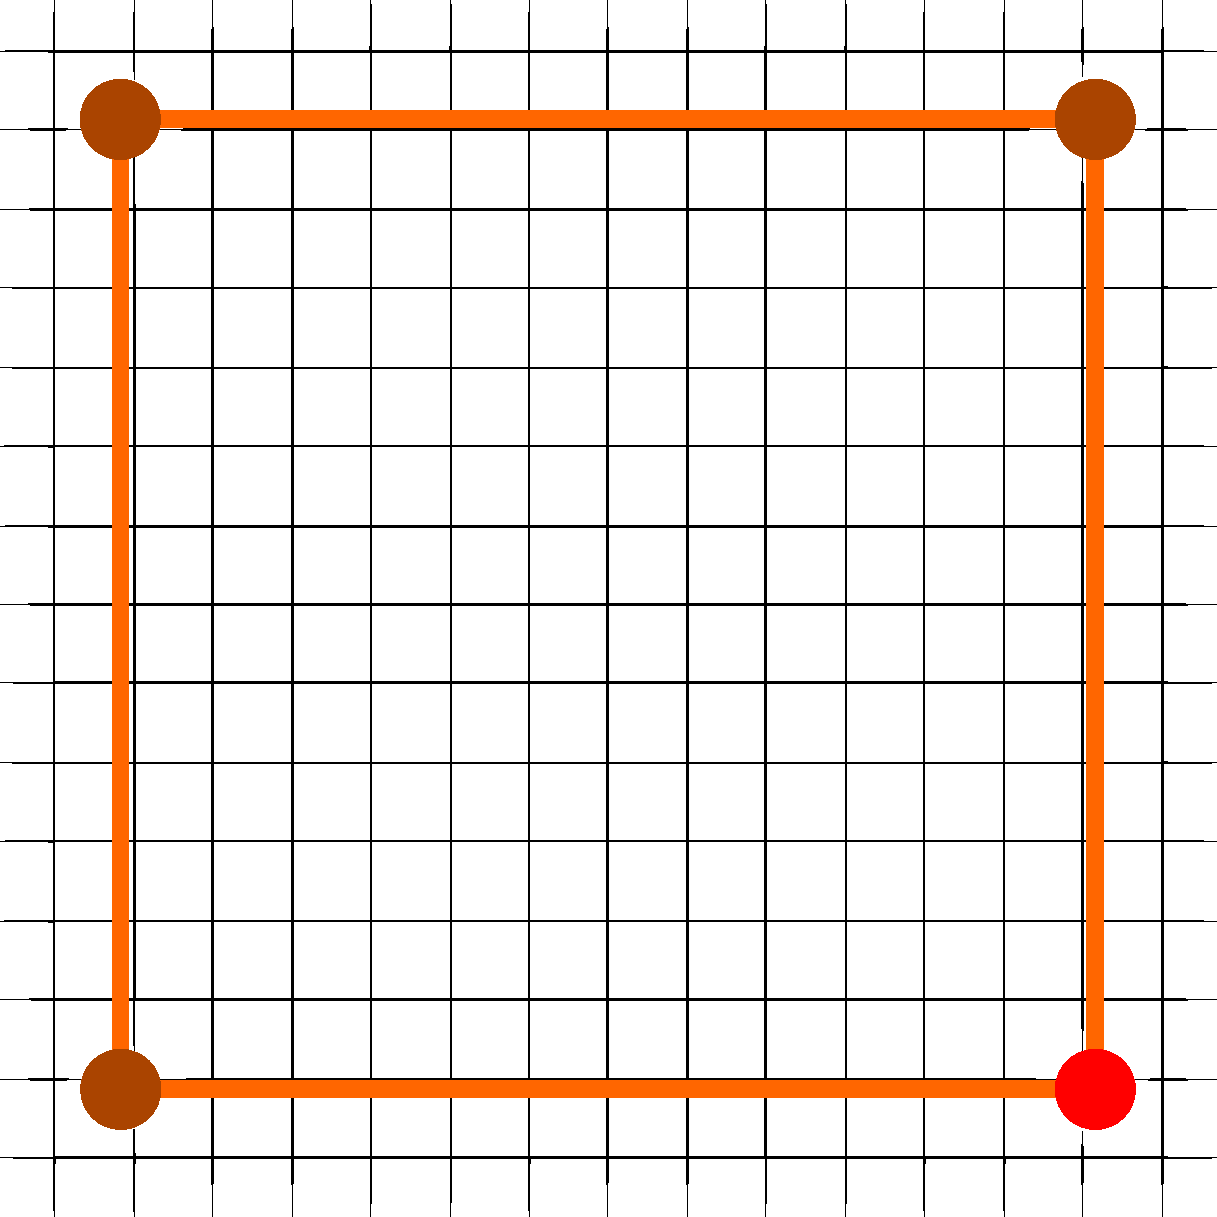
\includegraphics[scale=2]{Deformation-Interieur-1Sommet-Avant}
      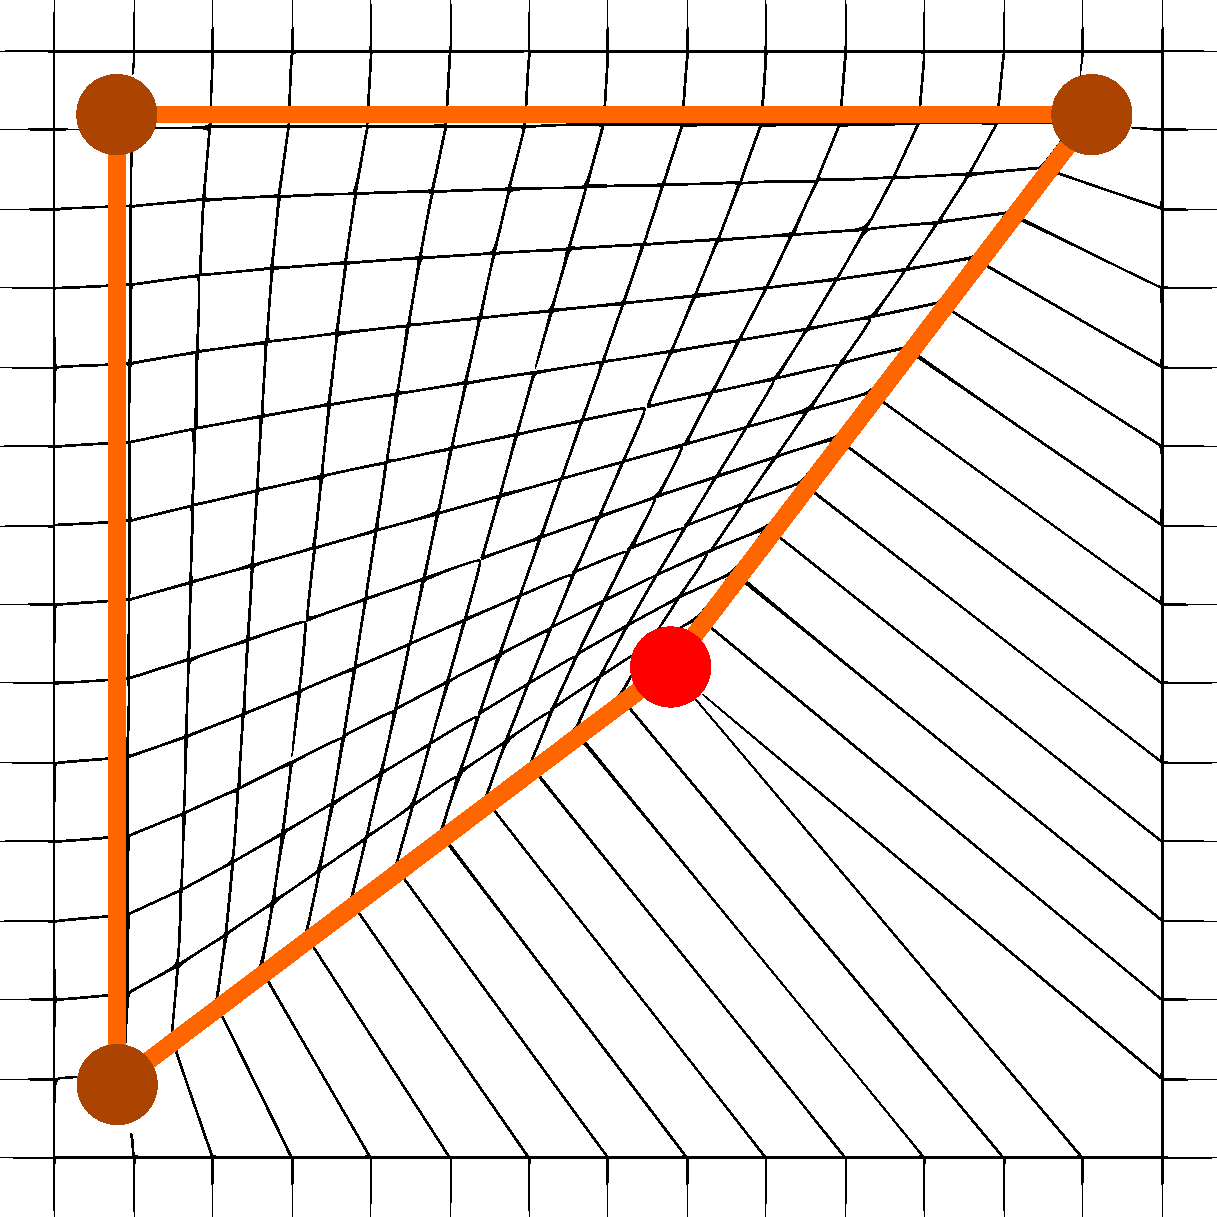
\includegraphics[scale=2]{Deformation-Interieur-1Sommet-Apres}
    }

    \caption[Problème de continuité déformation naïve] {Visualisation des
problèmes de continuité lorsque seuls les points à l'intérieur de la cage sont
déformés. Le bord de la cage est représenté en orange, l'objet est représenté
par une grille régulière en noir. Le sommet en rouge représente le sommet
déplacé. A gauche l'objet avant déformation, à droite le même objet après
déformation.}

    \label{MELVI}
  \end{center}
\end{figure}

En considérant des coordonnées pour les points de l'espace à la fois à
l'intérieur et à l'extérieur de la cage le problème vient de la dérivabilité
de la fonction résultant de la déformation. Plus précisément, pour les MVC et
GC la fonction de déformation est définie dans $\mathbb{R}^2$ et est
$C^{\infty}$ sauf au niveau des sommets de la cage où elle n'est que
$C^0$ (d'après \cite{LS08}). La déformation engendrée n'est pas visuellement lisse autour des
sommets de la cage. Quant aux HC, elles ne sont définies qu'à l'intérieur de
la cage où elles sont $C^{\infty}$. Il n'y a donc aucun moyen de déformer
l'extérieur de la cage de cette manière.

Notre objectif est d'obtenir une fonction de déformation, définie par une
cage, qui soit au moins $C^1$ partout (visuellement lisse) et dont la zone
d'influence soit limitée.

Plutôt que de mettre en place une nouvelle méthode de calcul de coordonnées
ayant les propriétés que nous souhaitons, ce qui au demeurant serait un sujet
de recherche en soi, nous nous intéressons à la réutilisation des méthodes de
calcul existantes.

\subsubsection{Principe}

Nous considérons deux cages là où les travaux antérieurs n'en considéraient
qu'une seule. Nous appelons \textit{cage de contrôle} la cage avec laquelle
l'utilisateur interagit pour réaliser les déformations. Nous appelons
\textit{cage d'influence} la cage qui définit la zone d'influence (points de
l'espace qui sont sous l'influence de la déformation). La cage d'influence est
homothétique à la cage de contrôle et contient strictement cette dernière
(Figure \ref{MELDou}). Pour simplifier les écritures dans la suite du travail,
nous nous référons à l'outil composé d'une cage de contrôle et d'une cage
d'influence comme l'outil \textit{double-cage}.

\begin{figure}[ht]
  \begin{center}
    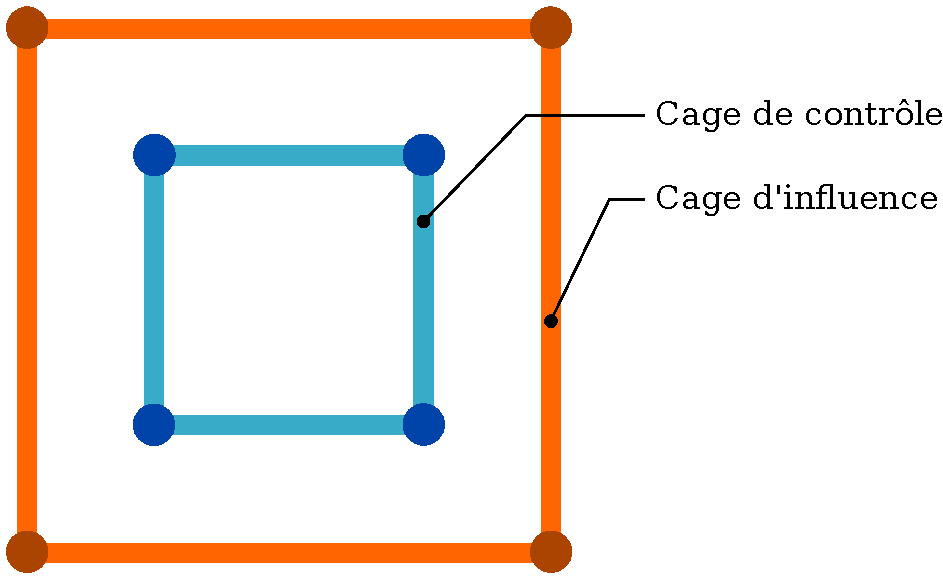
\includegraphics[scale=0.4]{chapter3-doubleCage-description-pstricks}

    \caption[Disposition des cages de contrôle et d'influence] {Disposition
des deux cages. En bleu la cage de contrôle, en orange la cage d'influence.}

    \label{MELDou}
  \end{center}
\end{figure}

Avec cette disposition, une partie de l'extérieur de la cage de contrôle est à
l'intérieur de la cage d'influence. Comme les coordonnées MVC sont
$C^{\infty}$ à l'intérieur de la cage d'influence (par définition). Les
déformations qui ont lieu à l'intérieur de celle-ci sont donc visuellement
lisses. Nous introduisons une notion de hiérarchie de déformation, où la
modification de la position des sommets de la cage de contrôle va modifier la
position des sommets de la cage d'influence, qui  elle-même va modifier
l'espace contenu en son intérieur quelque soit la méthode de calcul de
coordonnées (MVC, HC, GC). \\

\subsubsection{Hiérarchie de la déformation}

Il faut maintenant établir un lien entre les deux cages, afin que la
modification de la position des sommets de la cage de contrôle affecte la
position des sommets de la cage d'influence.

Une première idée est d'utiliser des coordonnées barycentriques généralisées
pour évaluer la position de chacun des sommets de la cage d'influence comme
une combinaison linéaire pondérée des positions des sommets de la cage de
contrôle. Cette technique pose le problème de la localité de la déformation :
la modification de la position d'un sommet de la cage de contrôle modifie la
position de tous les sommets de la cage d'influence (Figure \ref{MELDMV}).
Nous voulons que les points les plus éloignés du sommet modifié soient le
moins affectés par la déformation engendrée. La modification de la position
d'un sommet de la cage de contrôle doit donc modifier le moins de sommets de
la cage d'influence.

\begin{figure}[ht]
\begin{center}
  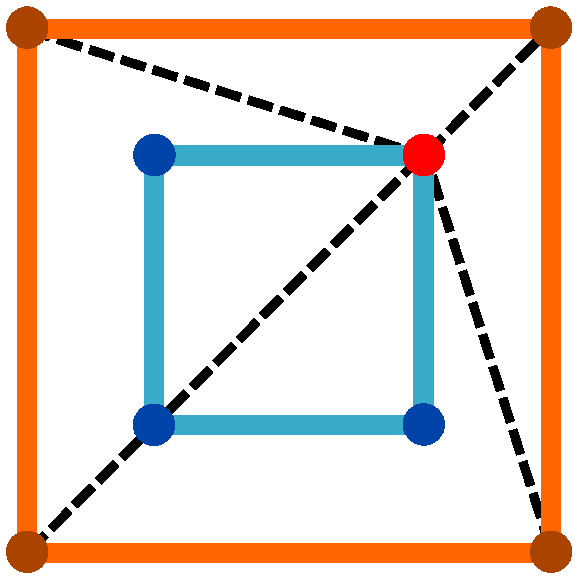
\includegraphics[scale=0.4]{chapter3-doubleCage-MVC-avant-pstricks}
  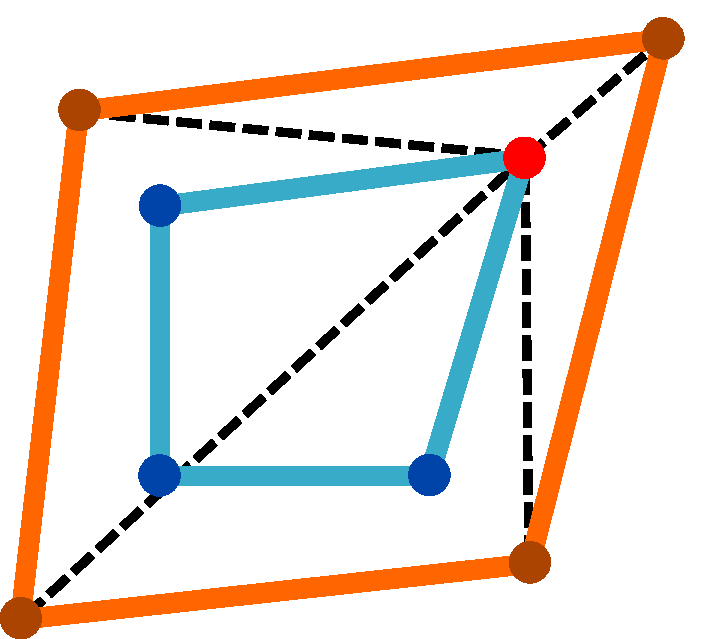
\includegraphics[scale=0.4]{chapter3-doubleCage-MVC-apres-pstricks}

  \caption[Lien double-cage MVC] {Lien entre les cages de contrôle et
d'influence utilisant les coordonnées MVC. Les pointillés noirs représentent
le lien entre un sommet de la cage de contrôle et les sommets de la cage
d'influence. On peut remarquer que la position de tous les sommets de la cage
d'influence est modifiée à la modification de la position du sommet en rouge.}

  \label{MELDMV}
\end{center}
\end{figure}

A la place, nous proposons que chaque sommet de la cage d'influence soit lié à
un seul sommet de la cage de contrôle. Etant donné que l'on construit la cage
d'influence comme une version mise à l'échelle de la cage de contrôle, nous
lions les sommets de la cage de contrôle à leur homologues "mis à l'échelle"
de la cage d'influence. Ainsi, quand la position d'un sommet de la cage de
contrôle est modifiée, la position d'un seul sommet de la cage d'influence est
modifiée (Figure \ref{MELHie}).

On définit le lien par un vecteur $\overrightarrow{v}$ représentant la
différence de position entre un sommet de la cage d'influence $v_{inf}$ par
rapport au sommet de la cage de contrôle $v_{ctrl}$ auquel il est associé :

\begin{displaymath}
  \overrightarrow{v} = v_{inf}-v_{ctrl}
\end{displaymath}

\begin{figure}[ht]
\begin{center}
  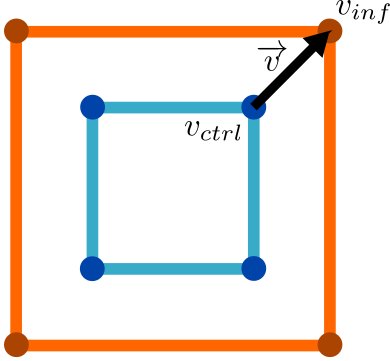
\includegraphics[scale=0.4]{chapter3-doubleCage-hierarchie-avant-pstricks}
  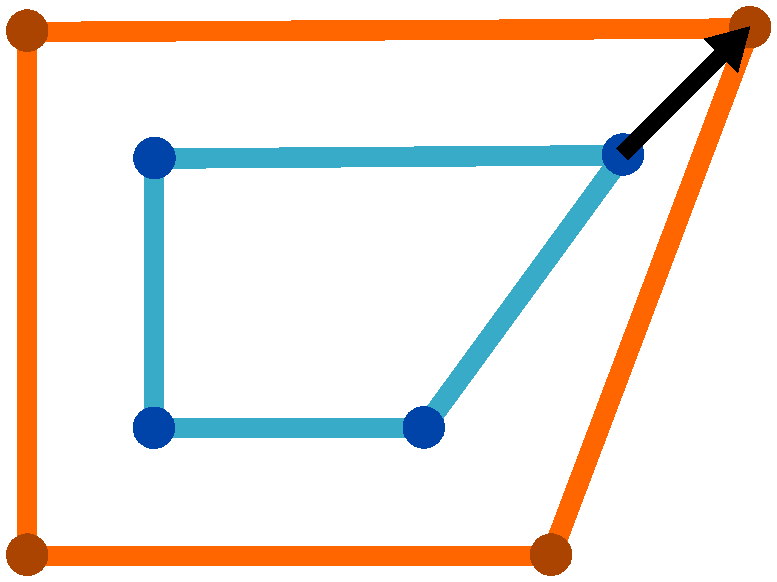
\includegraphics[scale=0.4]{chapter3-doubleCage-hierarchie-apres-pstricks}

  \caption[Association des cages de contrôle et d'influence] {Modification de
la position du sommet de la cage d'influence $v_{inf}$ associé au sommet de la
cage de contrôle déplacé $v_{ctrl}$. A gauche les cages avant déformation, à
droite les cages après déformation. En bleu la cage de contrôle, en orange la
cage d'influence et en noir le vecteur $v$.}

  \label{MELHie}
\end{center}
\end{figure}

\subsubsection{Atténuation de la déformation}

Pour l'instant, la déformation souffre toujours de problème de continuité au
niveau du bord de la cage d'influence. Pour corriger ce problème, nous
atténuons progressivement la déformation appliquée, en fonction de la distance
d'un point de l'espace au bord de la cage d'influence.

Pour atténuer la déformation nous avons choisi de réaliser une transformation
continue :

\begin{equation}
  T_{d}(p) = \gamma(p) T(p) + (1-\gamma(p)) p
  \label{MELAtt}
\end{equation}

où $T(p)$ correspond à la position que le point $p$ aurait après une déformation
classique, $p$ la position initiale du point et $T_{d}(p)$ la position finale
du point.

\textbf{Distance au bord de la cage d'influence :}

Nous avons choisi d'interpréter la fonction $\gamma$ comme représentant la
distance du point $p$ au bord de la cage d'influence. Nous utilisons les
coordonnées que nous avons déjà calculé pour chacun des points de l'espace par
rapport aux sommets de la cage d'influence. Ce choix a l'avantage de ne pas
nécessiter de calculs supplémentaires. Nous introduisons une distance au bord
$d_{inf}(p)$ qui est égale au produit des poids associés à chacune des arêtes
$e$ de la cage d'influence $c_{inf}$ :

\begin{equation}
  d_{inf}(p) = \prod_{e \in c_{inf}} (1 - \sum_{v_j \in e} \lambda_j(p))
  \label{MELInf}
\end{equation}

Ce calcul s'inspire de la notion de "boundary weight function" de
\cite{GPCP13}, utilisée pour évaluer la distance d'un point à chacune des
arêtes d'une cage.

De base, les valeurs de $d_{inf}(p)$ sont comprises dans l'intervalle
$[0,(\frac{2}{n})^n]$ où $n$ représente le nombre de sommets de la cage
d'influence. Pour utiliser cette fonction comme interpolant dans l'équation
\ref{MELAtt}, il faut normaliser l'ensemble de ses valeurs pour qu'elles
soient comprises dans l'intervalle $[0,1]$. Pour cela on divise l'ensemble des
valeurs de $d_{inf}(p)$ par $(\frac{2}{n})^n$.

Illustrons cette fonction par quelques exemples afin de mieux comprendre son
utilité :

\textit{Exemple 1 :} Soit $p$ le centre de gravité de la cage d'influence
(Figure \ref{MELEx1}).

\begin{figure}[ht]
\begin{center}
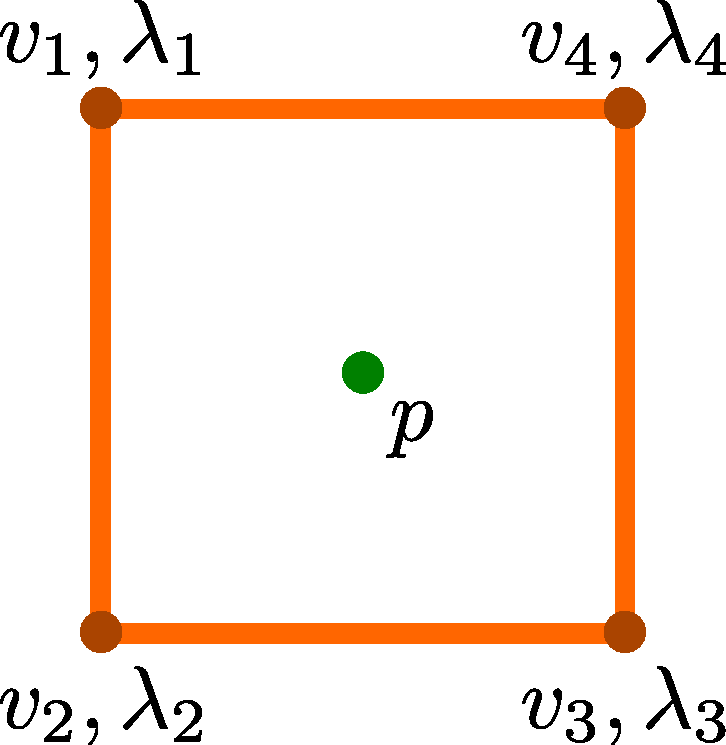
\includegraphics[scale=0.4]{Deformation-Attenuation-Exemple1}

\caption[Atténuation : Exemple 1] {En orange la cage de contrôle, en bleu la
cage d'influence et en vert le point de l'espace $p$ considéré. $p$ est le
centre de gravité de la cage d'influence, toutes ses coordonnées $\lambda_i$
sont donc égales.}

\label{MELEx1}
\end{center}
\end{figure}

\begin{center}
\fbox{\begin{minipage}{1.\textwidth}
Les coordonnées $\lambda_i$ qui lui sont attribuées sont toutes égales (par
définition) : $\lambda_1 = \lambda_2 = \lambda_3 = \lambda_4 = \frac{1}{4}$.
Sa distance au bord de la cage d'influence vaut donc:
\begin{displaymath}
  d_{inf}(p) = \frac{(1 - (\lambda_1 + \lambda_2)) * (1 - (\lambda_2 + \lambda_3)) 
* (1 - (\lambda_3 + \lambda_4)) * (1 - (\lambda_4 + \lambda_1))}{(2/4)^4},
\end{displaymath}

en remplaçant par les valeurs numériques, on obtient :
\begin{displaymath}
  d_{inf}(p) = 1.
\end{displaymath}

Donc pour un point $p$ situé au centre de gravité de la cage d'influence, sa
distance au bord $d_{inf}(p)$ vaut 1, cela signifie qu'il n'y a pas de point
plus éloigné du bord (par définition de la fonction), ce qui est cohérent
avec la construction du point $p$.
\end{minipage}}
\end{center}

\textit{Exemple 2 :} 

Soit $q$ un point de l'espace se situant sur le bord de la cage d'influence,
sur l'arête formée par les sommets $v_4$ et $v_1$ (Figure \ref{MELEx2}).

\begin{figure}[ht]
\begin{center}
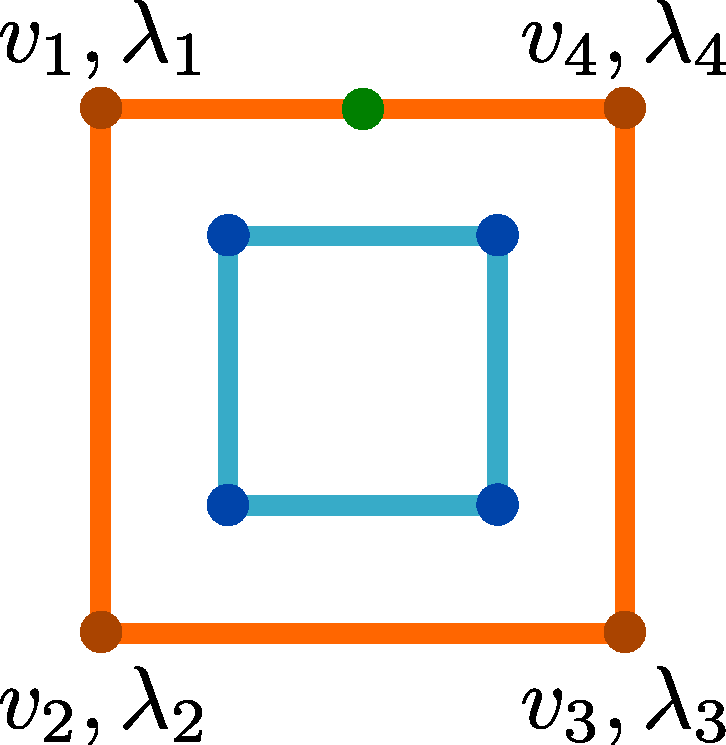
\includegraphics[scale=0.4]{Deformation-Attenuation-Exemple2}

\caption[Atténuation : Exemple 2] {En orange la cage de contrôle, en bleu la cage d'influence
et en vert le point de l'espace $q$ considéré. $q$ se situe sur le bord de la
cage d'influence, entre les sommets $v_4$ et $v_1$.}

\label{MELEx2}
\end{center}
\end{figure}

\begin{center}
\fbox{\begin{minipage}{1.\textwidth}
Par définition, comme les coordonnées évoluent de façon linéaire le long des
arêtes de la cage $v_2$ et $v_3$ n'ont aucune influence sur la position de
$p$. Autrement dit : $\lambda_2 = \lambda_3 = 0$ et $\lambda_1 +
\lambda_4 = 1$ (car $\sum_i \lambda_i = 1$). On en déduit :
\begin{displaymath}
d_{inf}(p) = \frac{(1 - (\lambda_1 + \lambda_2)) * (1 - (\lambda_2 + \lambda_3)) 
* (1 - (\lambda_3 + \lambda_4)) * (1 - (\lambda_4 + \lambda_1))}{(\frac{2}{4})^4},
\end{displaymath}

comme $\lambda_1 + \lambda_4 = 1$, on obtient :
\begin{displaymath}
d_{inf}(p) = 0.
\end{displaymath}

La distance au bord d'un point $p$ situé sur une arête de la cage d'influence
vaut 0, cela signifie que $p$ est sur le bord de la cage (par définition de la
fonction), ce qui est cohérent avec la construction du point $p$.
\end{minipage}}
\end{center}

La fonction $d_{inf}(p)$ n'est pas dérivable aux extrémités de la cage d'influence
(Figure \ref{MELAtN}). La fonction $\gamma(p)$ ne peut donc pas être
directement égale à $d_{inf}(p)$.

\begin{figure}[ht]
\begin{center}
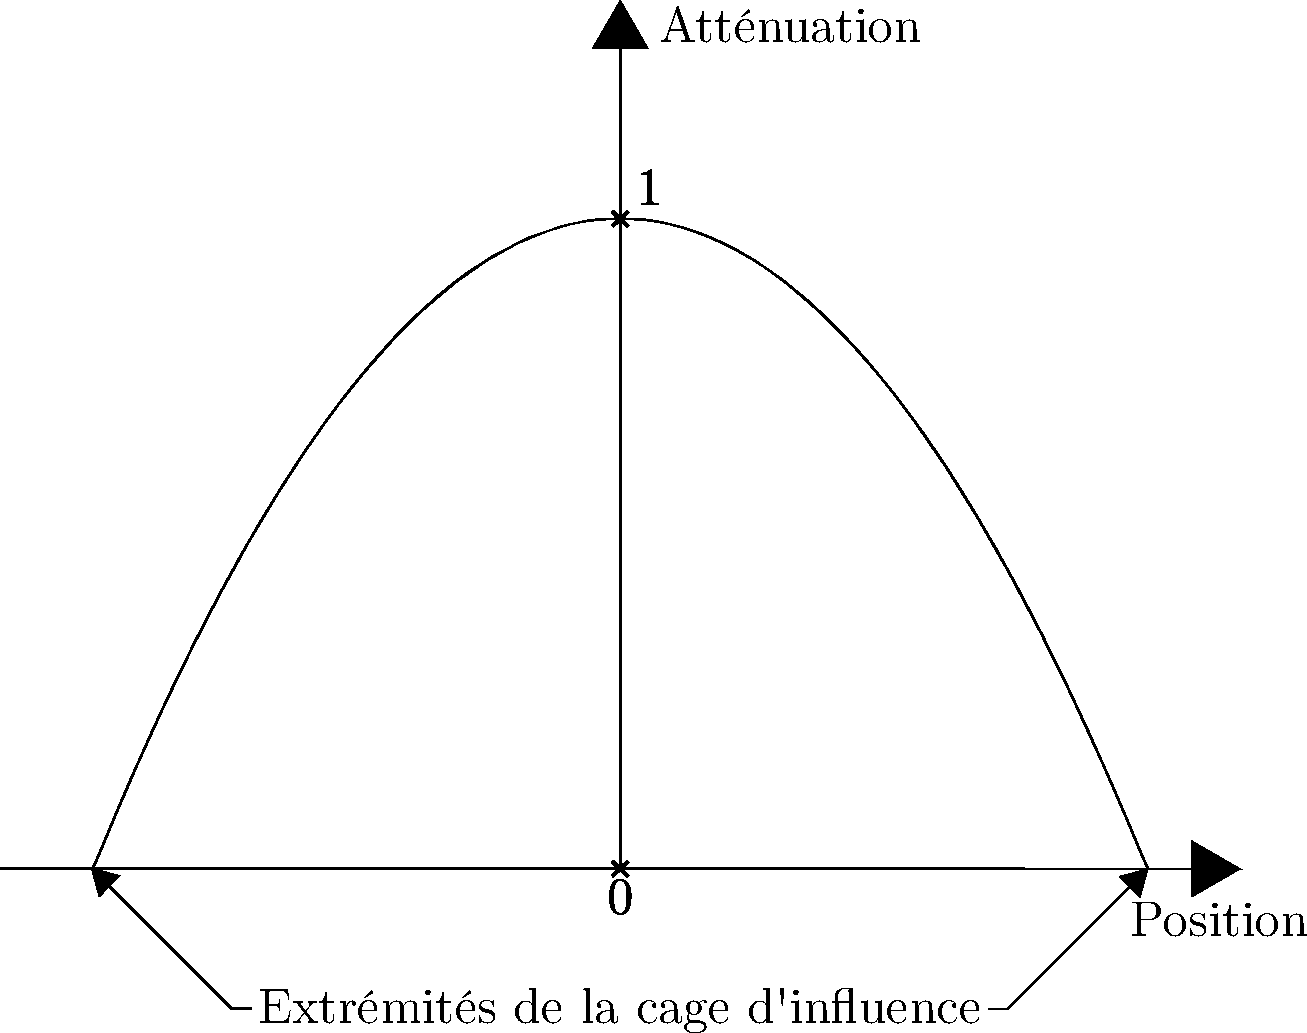
\includegraphics[scale=0.4]{Fonction-Attenuation-Sans}

\caption[Fonction d'atténuation $d_{inf}(p)$] {Vue en coupe (au centre de
gravité de la cage d'influence) de la fonction d'atténuation $d_{inf}(p)$. On
remarque que la fonction n'est pas dérivable au niveau des extrémités de la
cage d'influence.}

\label{MELAtN}

\end{center}
\end{figure}

\newpage

\textbf{Lissage de la fonction d'atténuation $d_{inf}(p)$ :}

L'idée vient du travail de \cite{GPCP13}. une fonction pour lisser les
valeurs de distance d'un point à une arête de la cage. Considérons une
fonction $f_h(x)$, paramétrée par $h \in ]0, 1]$, permettant de lisser les
valeurs des distances des points de l'espace au bord de la cage d'influence
$d_{inf}(p)$. Cette fonction doit satisfaire $f_h(0) = f_h'(0) = f_h'(1) = 0$,
$f_h(x)=1$ pour $x \geq h$ et $f_h(x) \geq 0$, afin d'obtenir une notion de
continuité au niveau du raccord entre les points de l'espace affectés par la
déformation et ceux qui ne le sont pas. Cette fonction va directement
normaliser les valeurs pour qu'elles soient comprises dans l'intervalle
$[0,1]$, il n'est donc plus nécessaire de diviser par $(\frac{2}{n})^n$. Les
auteurs proposaient plusieurs fonctions avec des comportements similaires,
après les avoir testées, nous avons choisi d'en garder une en particulier sur
un critère de minimisation de temps de calcul :

\begin{equation}
  f_h(x) = \frac{1}{2} sin(\pi(\frac{x}{h} - \frac{1}{2})) + \frac{1}{2}
\end{equation}

\textbf{Calcul du paramètre $h$ :}

Il faut évaluer la valeur de $h$ de manière à ce que ce paramètre représente
la différence de taille entre la cage de contrôle et la cage d'influence. Nous
souhaitons que la déformation ne soit pas atténuée pour l'ensemble des points
de l'espace à l'intérieur de la cage de contrôle. Pour cela nous définissons
$h$ comme étant la plus courte distance d'un point contenu dans la cage de
contrôle au bord de la cage d'influence. Il se trouve que c'est exactement la
distance du sommet de la cage de contrôle le plus proche de la cage
d'influence (par construction). Il nous suffit donc d'évaluer la valeur de
distance en chacun des sommets de la cage de contrôle par rapport au bord de
la cage d'influence et de les comparer afin de trouver la distance minimale:

\begin{equation}
  h = \min_{\forall v_{ctrl}} d_{inf}(v_{ctrl}),
\end{equation}

où $v_{ctrl}$ correspond à un sommet de la cage de contrôle. L'espace est à
présent découpé en 3 sous-ensembles : 

\begin{itemize}

\item l'intérieur de la cage de contrôle, où la déformation n'est pas atténuée,

\item la zone résultant de la différence entre la cage d'influence et la cage
de contrôle, où la déformation est progressivement atténuée en fonction de la
distance au bord de la cage d'influence,

\item l'extérieur de la cage d'influence, où la déformation n'est pas
appliquée.

\end{itemize}

Nous pouvons maintenant écrire $\gamma(p)$ comme étant le résultat du lissage
de la fonction \ref{MELInf} :

\begin{equation}
  \gamma(p) = f_h(d_{inf}(p)),
\end{equation}

où $h$ correspond à la distance du sommet de la cage de contrôle le plus
proche du bord de la cage d'influence, sa valeur est constante. Nous
remarquons qu'il n'y a plus de problèmes de continuité au niveau du bord de la
cage d'influence pour la fonction $\gamma(p)$ (Figure \ref{MELAtL}).

\begin{figure}[ht]
\begin{center}
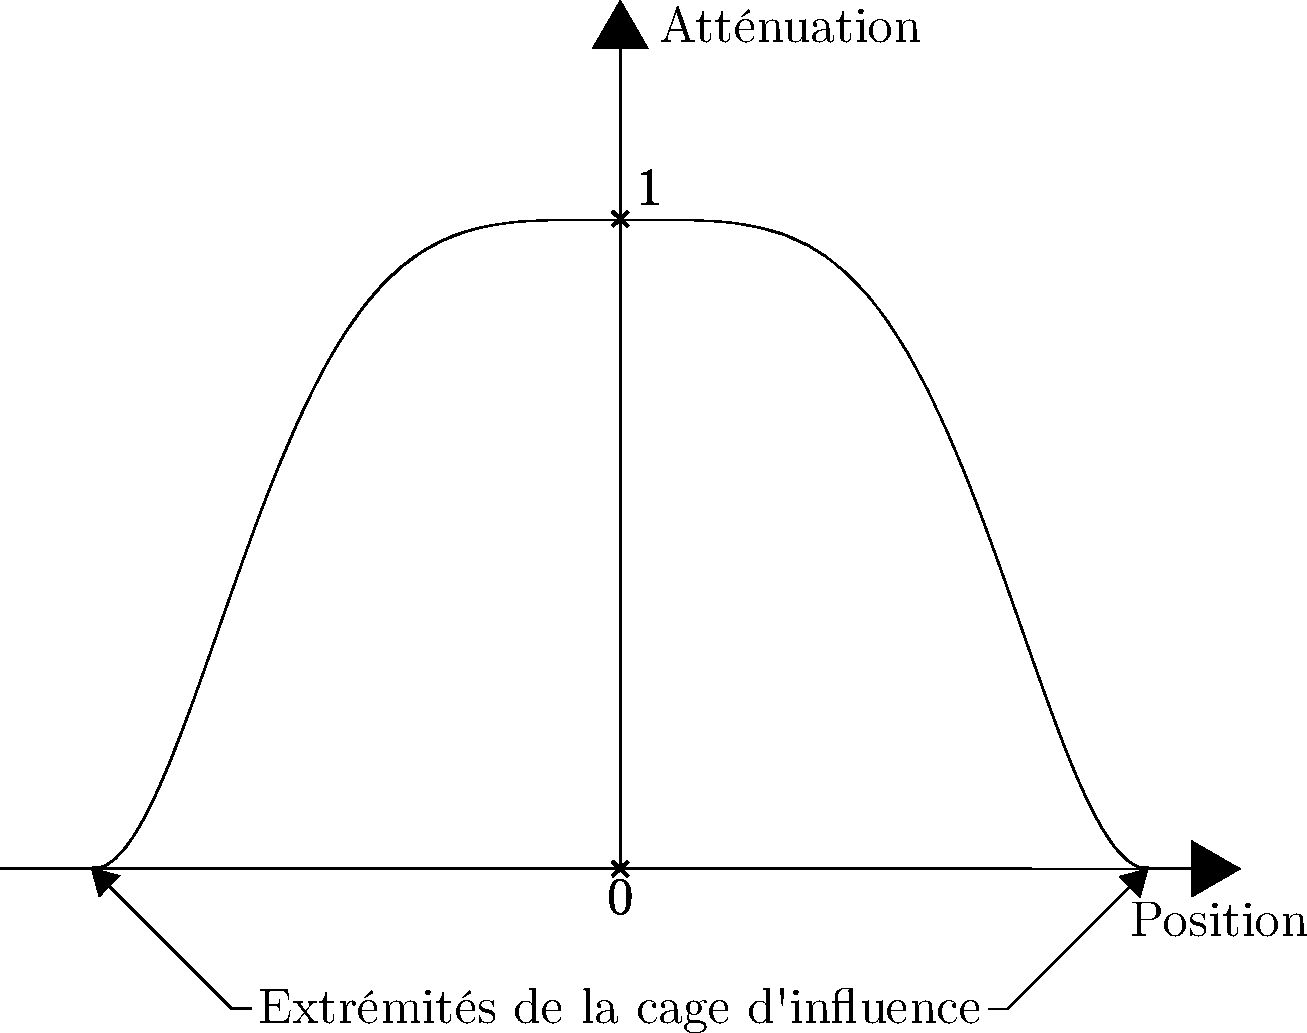
\includegraphics[scale=0.4]{Fonction-Attenuation-Avec}

\caption[Fonction d'atténuation $\gamma$(p)] {Vue en coupe (au centre de
gravité de la cage d'influence) de la fonction d'atténuation $\gamma(p)$. On
remarque que la fonction est maintenant dérivable au niveau des extrémités de
la cage d'influence.}

\label{MELAtL}

\end{center}
\end{figure}

Plus la différence de taille entre la cage de contrôle et la cage d'influence
est grande, plus l'atténuation de la déformation est douce (Figure
\ref{MELBou}).

\begin{figure}[ht]
  \begin{center}
    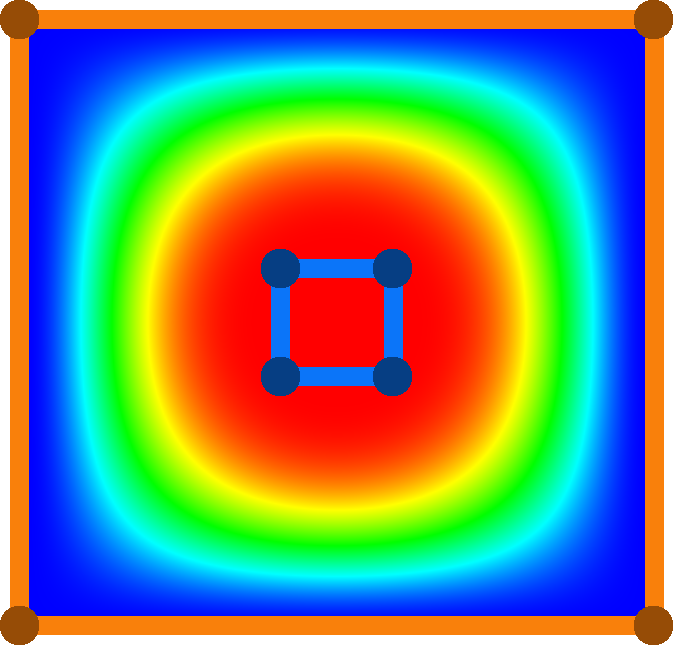
\includegraphics[scale=0.2]{BoundaryWeightFunction-Petite}
    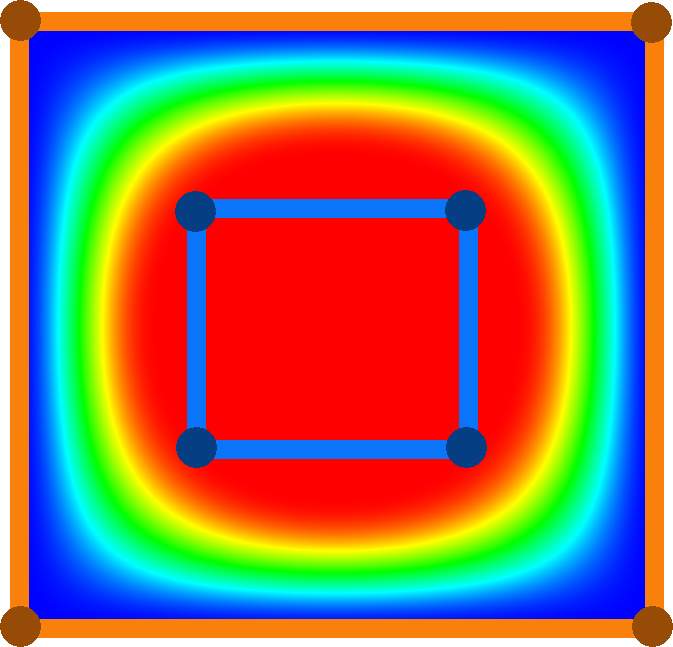
\includegraphics[scale=0.2]{BoundaryWeightFunction}
    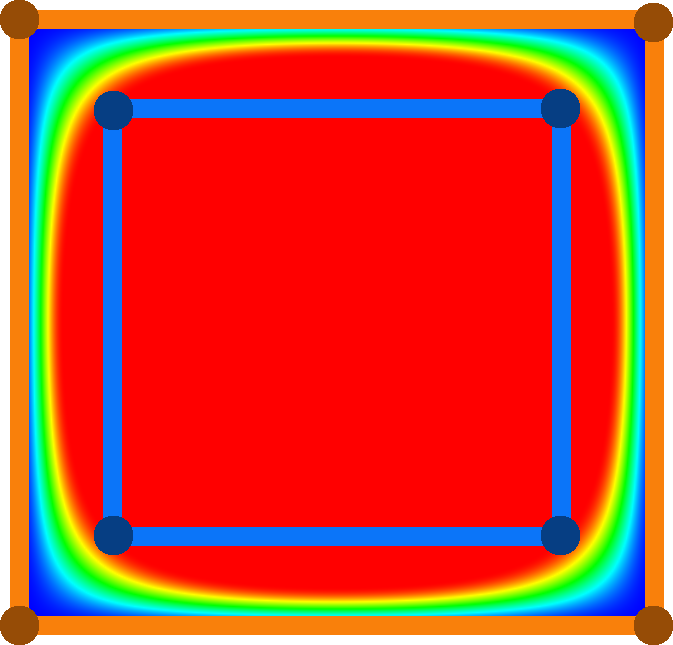
\includegraphics[scale=0.2]{BoundaryWeightFunction-Grande}

    \caption[Variation de l'atténuation de la déformation] {Variation de
l'atténuation de la déformation. La couleur varie du rouge (atténuation nulle)
au bleu (atténuation totale). De gauche à droite nous obtenons différentes
variations pour différentes tailles de cage de contrôle.}

    \label{MELBou}
  \end{center}
\end{figure}

Ci-dessous l'algorithme représentant l'étape de déformation de l'objet avec
atténuation de l'influence de la déformation: \\

\fbox{\begin{minipage}{0.9\textwidth}
  \begin{algorithm}[H]
  \KwIn{$pos$, $pos_{init}$ : tableau de tableau de réels}
  \ForEach{point de l'espace p}
  {
    $pos$[p] $\leftarrow$ [0,0]\; 
      \ForEach{sommet v de la cage d'influence c}
      {
        $pos$[p] $\leftarrow$ $pos$[p] + $\lambda_v(p)$ * $pos$[v] 
        * $\gamma(p)$\;
        $pos$[p] $\leftarrow$ $pos$[p] + $\lambda_v(p)$ * $pos_{init}$[v] 
        * (1-$\gamma(p)$)\;
      }
  }
  \caption{Déformation avec zone d'influence modifiée}
  \end{algorithm}
\end{minipage}}

\begin{figure}[ht]
  \begin{center}
    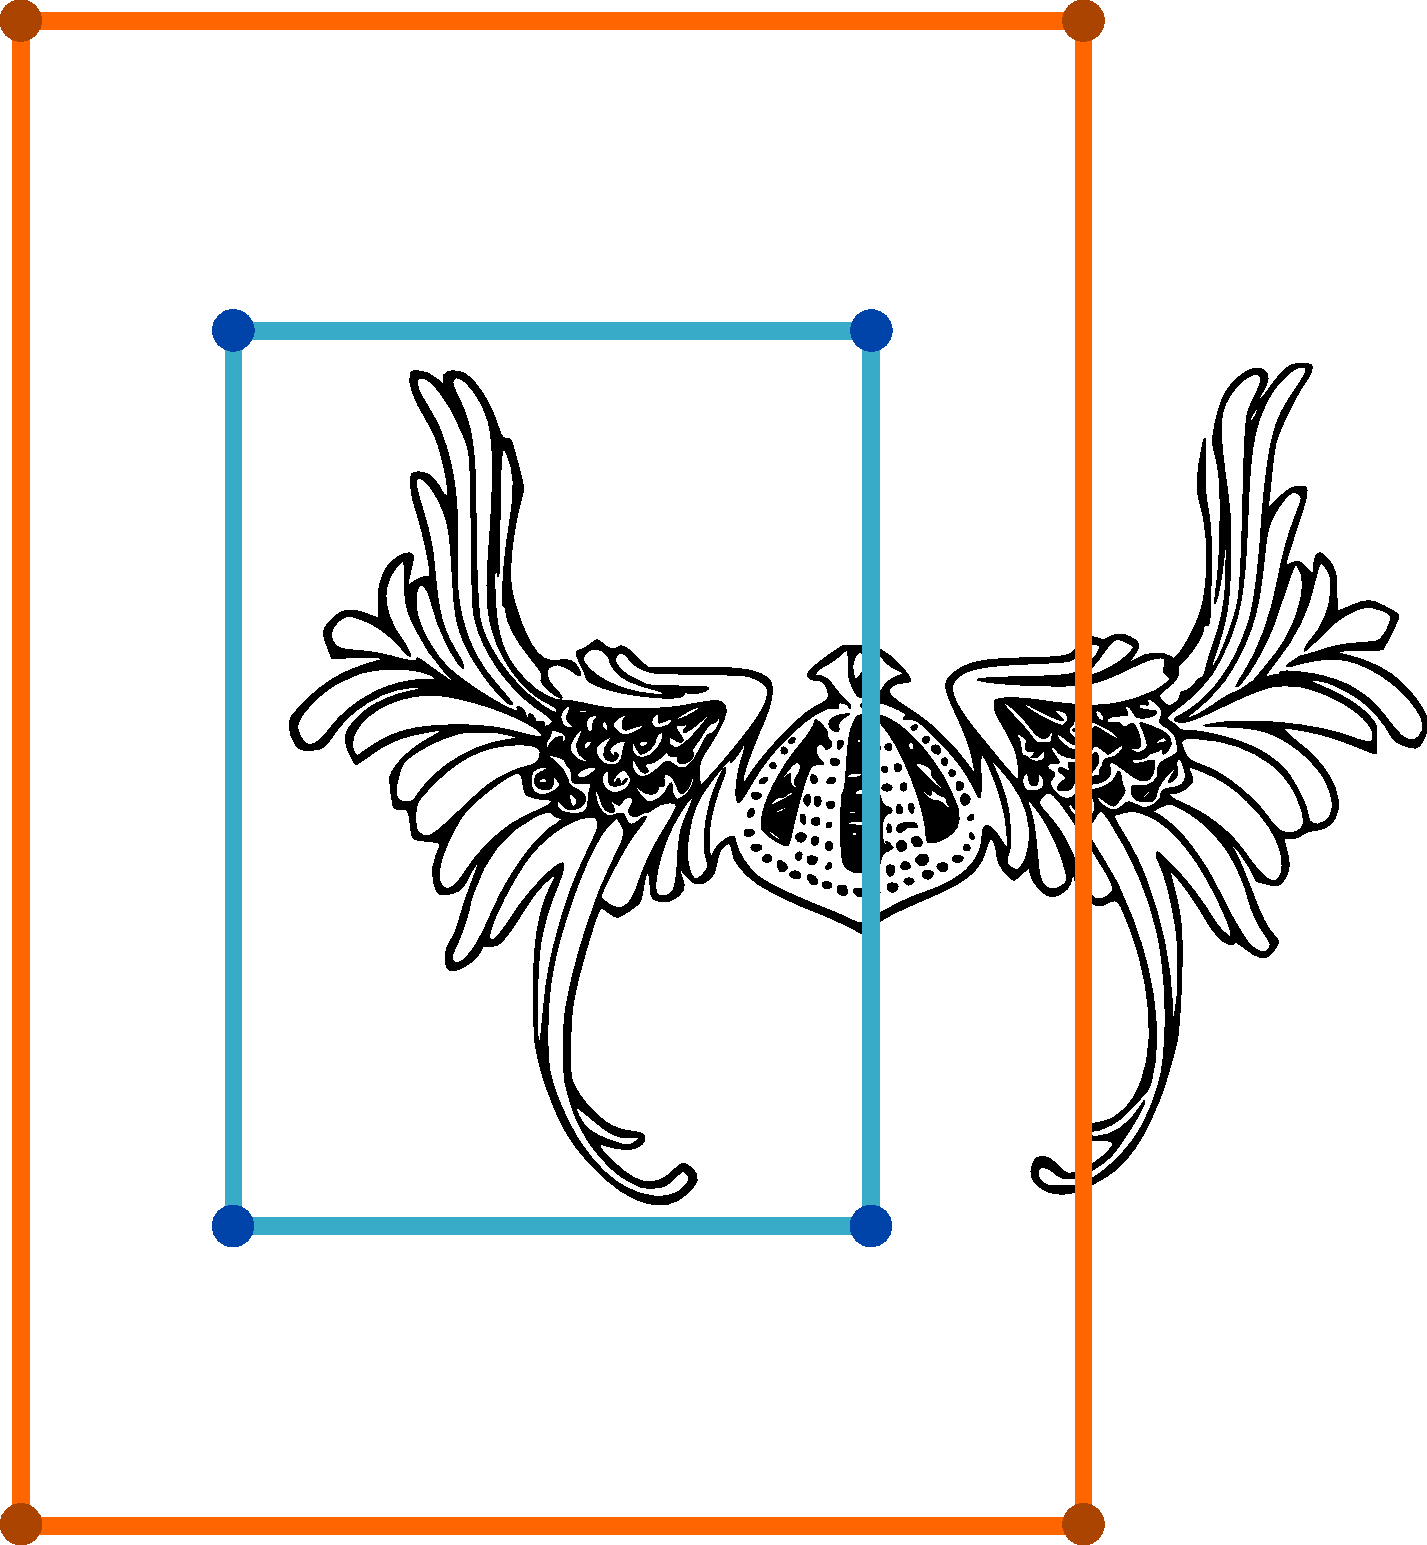
\includegraphics[scale=0.19]{Deformation-Viking-DoubleCage-Avant}\\
    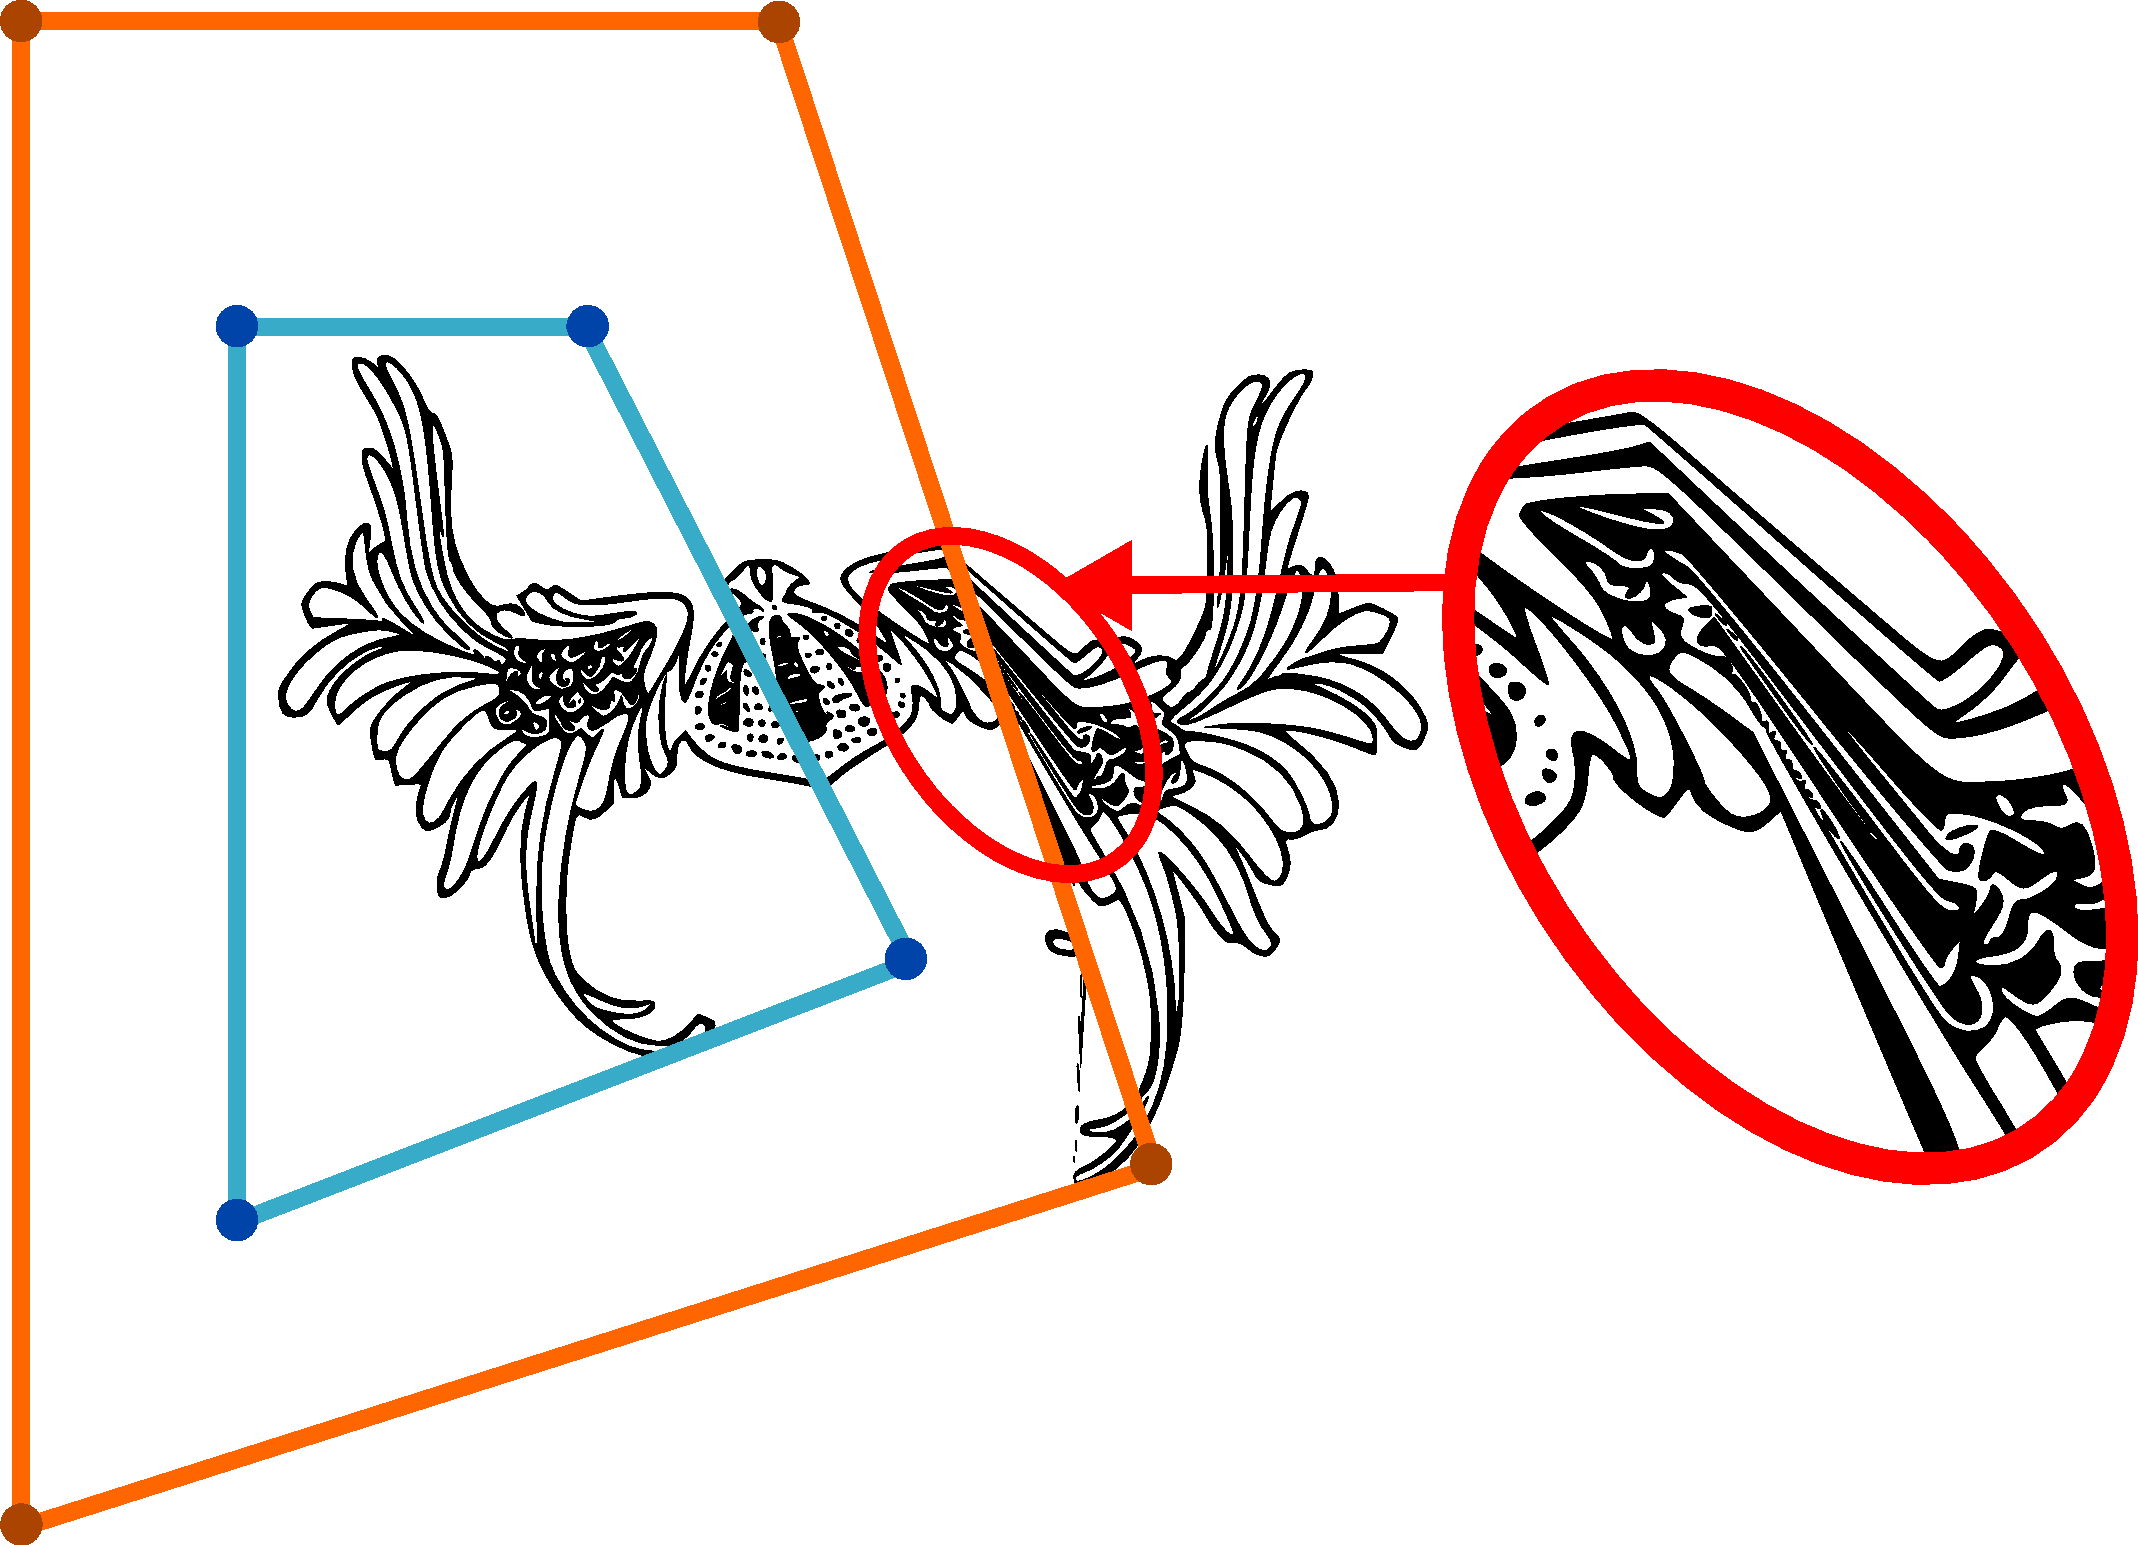
\includegraphics[scale=0.19]{Deformation-Viking-DoubleCage-Sans}
    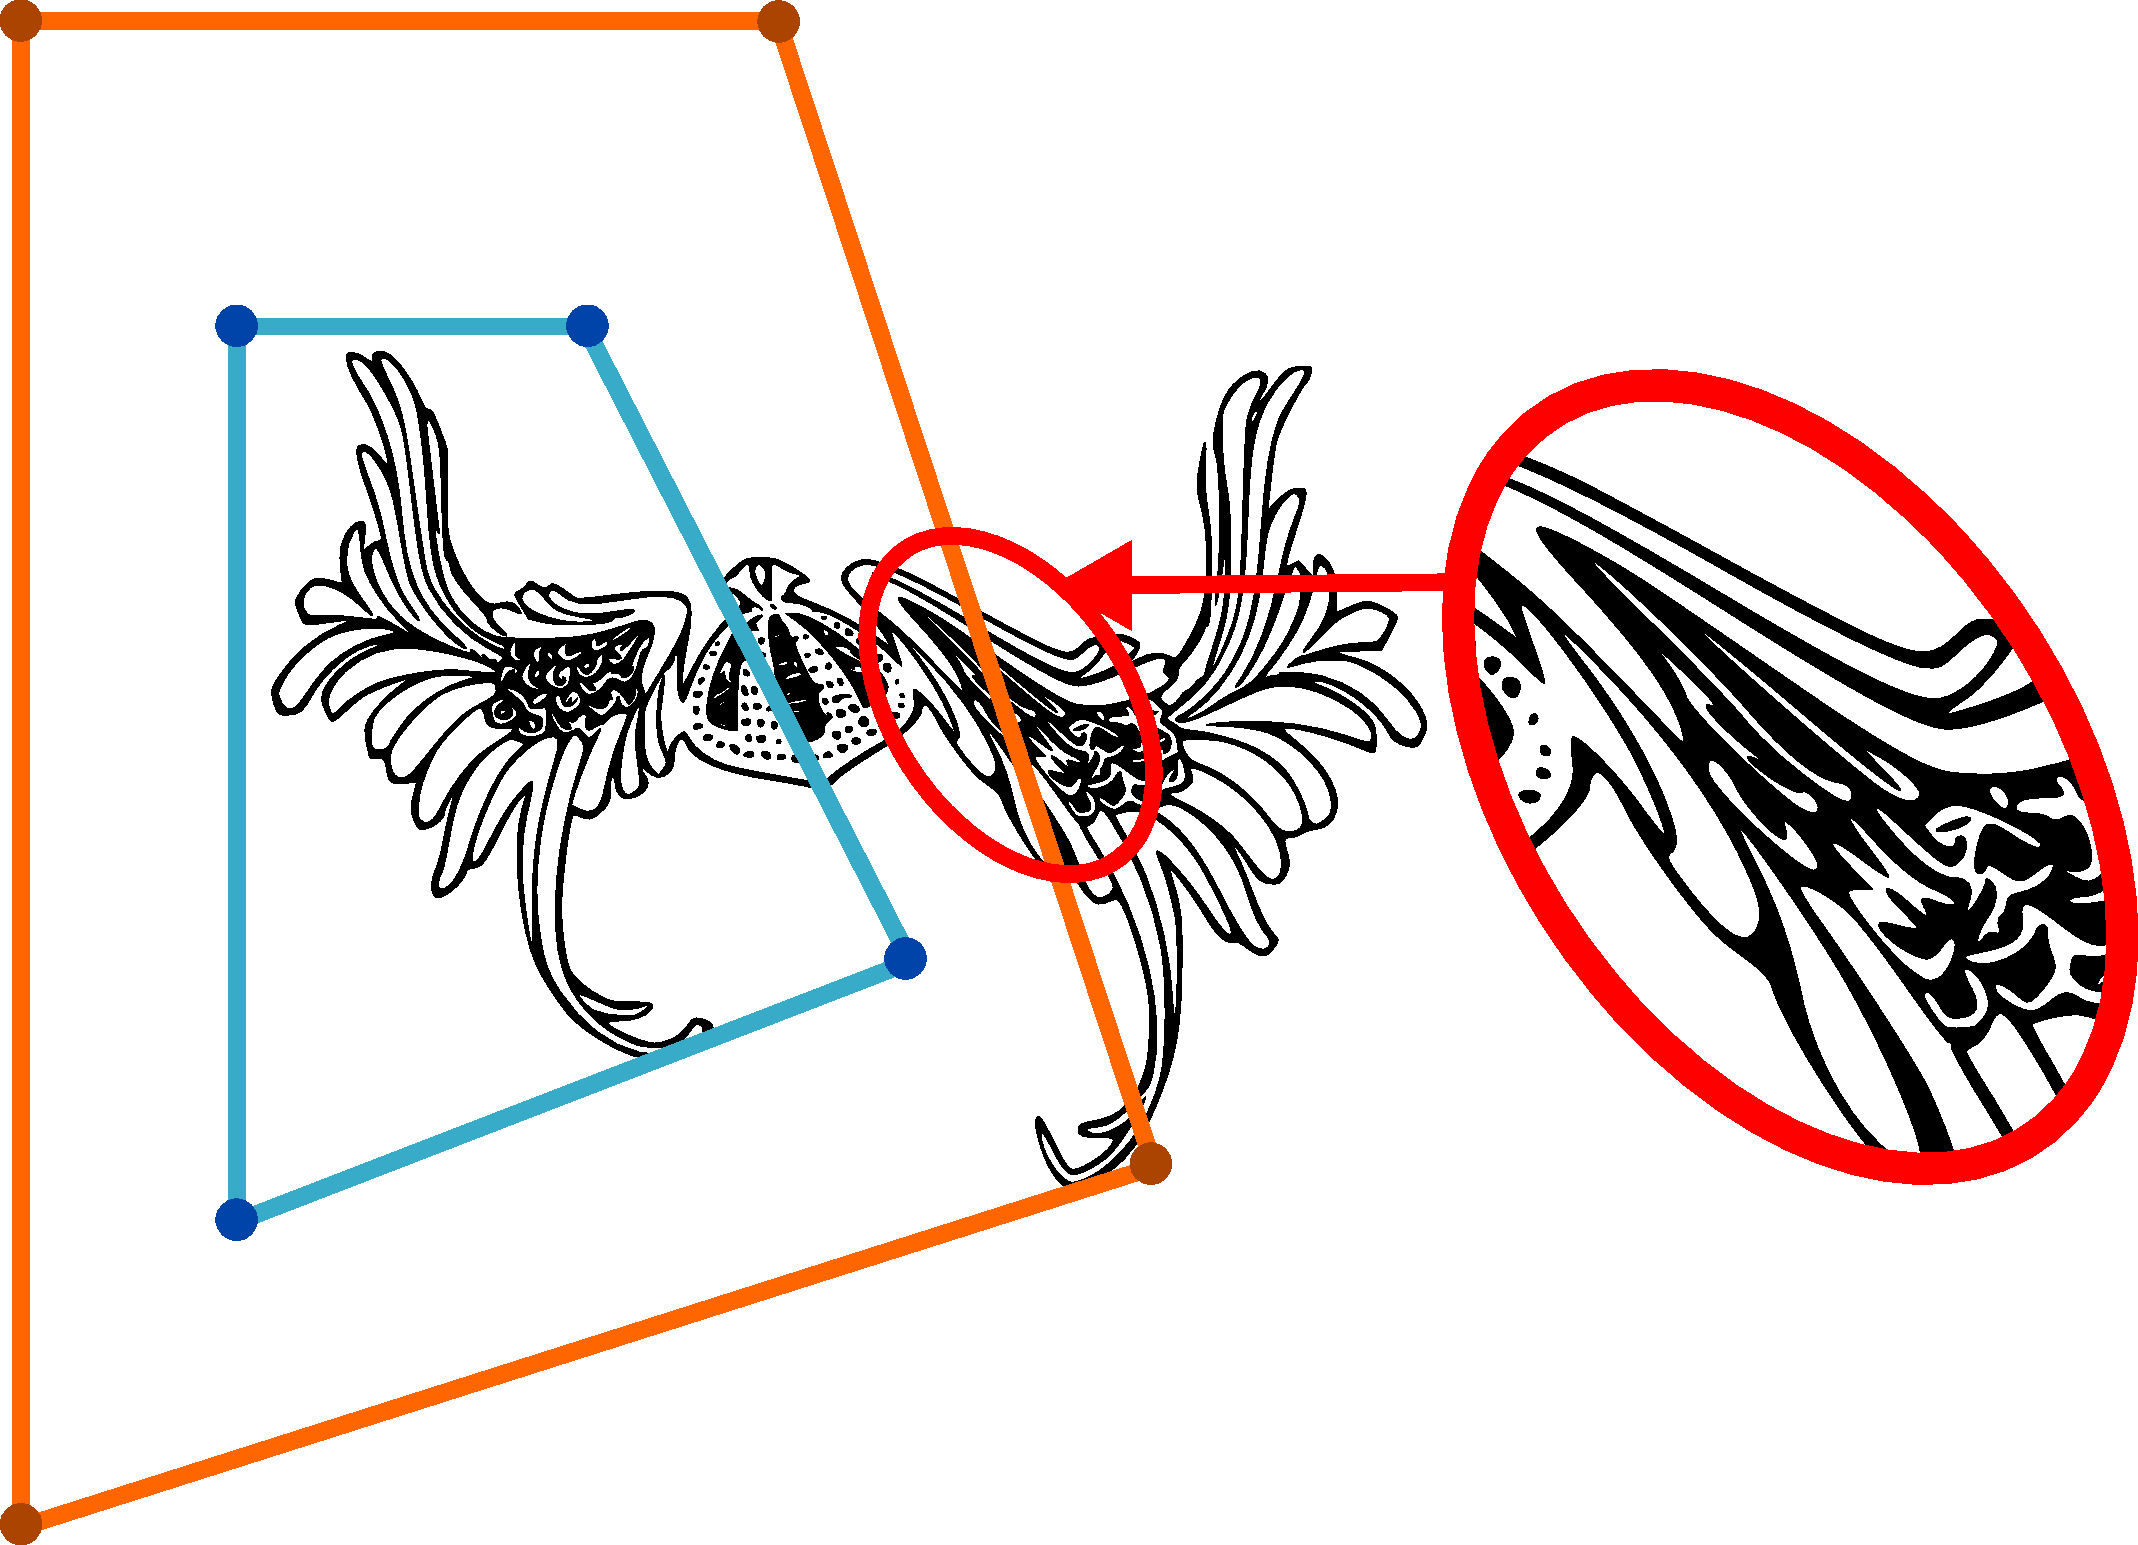
\includegraphics[scale=0.19]{Deformation-Viking-DoubleCage-Avec}

    \caption[Exemple de déformation double-cage] {Exemple de déformation avec
une double-cage (en bleu la cage de contrôle, en orange la cage d'influence).
En haut l'objet et la double-cage au temps d'association, en bas à gauche
sans atténuation, en bas à droite avec atténuation. On peut
remarquer que la déformation n'est pas visuellement lisse au bord de la cage
d'influence lors de la déformation sans atténuation.}

  \end{center}
\end{figure}

\subsection{Combinaison des déformations}

Maintenant que nous avons établi un outil de déformation local, nous voulons
combiner plusieurs double-cages sur un même objet (Figure \ref{MELMC}).
L'objectif de cette partie consiste à trouver une formule de mélange
permettant la modification de la position d'un point de l'espace sous
l'influence de plusieurs double-cages. De manière à ce que la déformation
résultant du mélange soit visuellement lisse.

\begin{figure}[ht]
  \begin{center}
    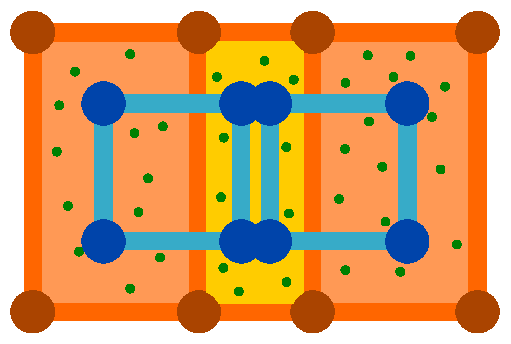
\includegraphics[scale=0.9]{chapter3-doubleCage-melange-pstricks}

    \caption[Mélange de double-cages] {Exemple de
configuration de deux double-cages se chevauchant. Les points
de l'espace (en vert) appartenant à la zone en jaune sont sous l'influence des
deux cages à la fois}

    \label{MELMC}
  \end{center}
\end{figure}

Combiner les déformations revient à établir une combinaison linéaire pondérée
de l'influence de chaque double-cage. Pour établir la valeur du coefficient
associé à chaque cage, il faut trouver un critère permettant de classer les
cages selon l'importance de la déformation à appliquer. Le critère que nous
décidons d'envisager est celui de distance. En effet, intuitivement, plus un
point de l'espace est proche du centre de gravité d'une double-cage, plus nous
voulons que cette cage influe sur la déformation de ce point. Autrement dit,
nous regardons la proximité d'un point de l'espace au centre de gravité de
chaque double-cage à laquelle il appartient.

Comparer la proximité au centre de gravité de gravité d'une double-cage
revient au même que de comparer l'éloignement au bord de la cage d'influence
(puisque nous ne considérons que des cages convexes). Ainsi, nous réutilisons
les valeurs de distance $d_{inf}(c, p)$ au bord de la cage d'influence
constituant la double- cage $c$ pour connaître la proximité d'un point au
centre de gravité de chaque double-cage dans laquelle il est inclus. Ces
distances étant relatives à chaque cage, il est nécessaire de les normaliser
afin de pouvoir les comparer entre elles :

\begin{displaymath}
  D(c, p) = \frac{\gamma(c, p)}{\sum_{j=0}^n d_{inf}(j, p)}, 
\end{displaymath}

où $D(c, p)$ correspond à la distance normalisée du point $p$ par rapport au
bord de la cage d'influence de la double-cage $c$.

On peut maintenant définir une fonction de mélange se basant sur la proximité
d'un point de l'espace au centre de gravité de chaque double-cage à laquelle
il appartient :

\begin{displaymath}
  T_{mel}(c, p) = \sum_{i=0}^n D(c, p) T_{d}(c, p),
\end{displaymath}

où $T_{d}(c, p)$ représente la position du point $p$ relativement à la double-
cage $c$

Ci-dessous l'algorithme représentant l'étape de déformation de l'objet avec le
mélange des déformations: \\

\fbox{\begin{minipage}{0.9\textwidth}
\begin{algorithm}[H]
\KwData{$sumD$, $D$: réel}
\KwIn{$pos$, $pos_{init}$ : tableau de tableau de réels}
\ForEach{point de l'espace p}
{
  $sumD$ $\leftarrow$ 0\;
  \ForEach{cage d'influence c associée à p}
  {
    $sumD$ $\leftarrow$ $sumD$ + $\gamma(c, p)$\;
  }
  $pos$[p] = [0,0]\; 
  \ForEach{cage d'influence c associée à p}
  {
    $D$ $\leftarrow$ $\gamma(c, p)$ / $sumD$\;
    \ForEach{sommet v de c}
    {
      $pos$[p] $\leftarrow$ $pos$[p] + $\lambda_v(p)$ * $pos$[v] 
      * $\gamma(c, p)$ * $D$\;
      $pos$[p] $\leftarrow$ $pos$[p] + $\lambda_v(p)$ * $pos_{init}$[v] 
      * (1-$\gamma(c, p)$) * $D$\;
    }
  }
}
\caption{Mélange des déformations}
\end{algorithm}
\end{minipage}}

\begin{figure}[ht]
  \begin{center}
    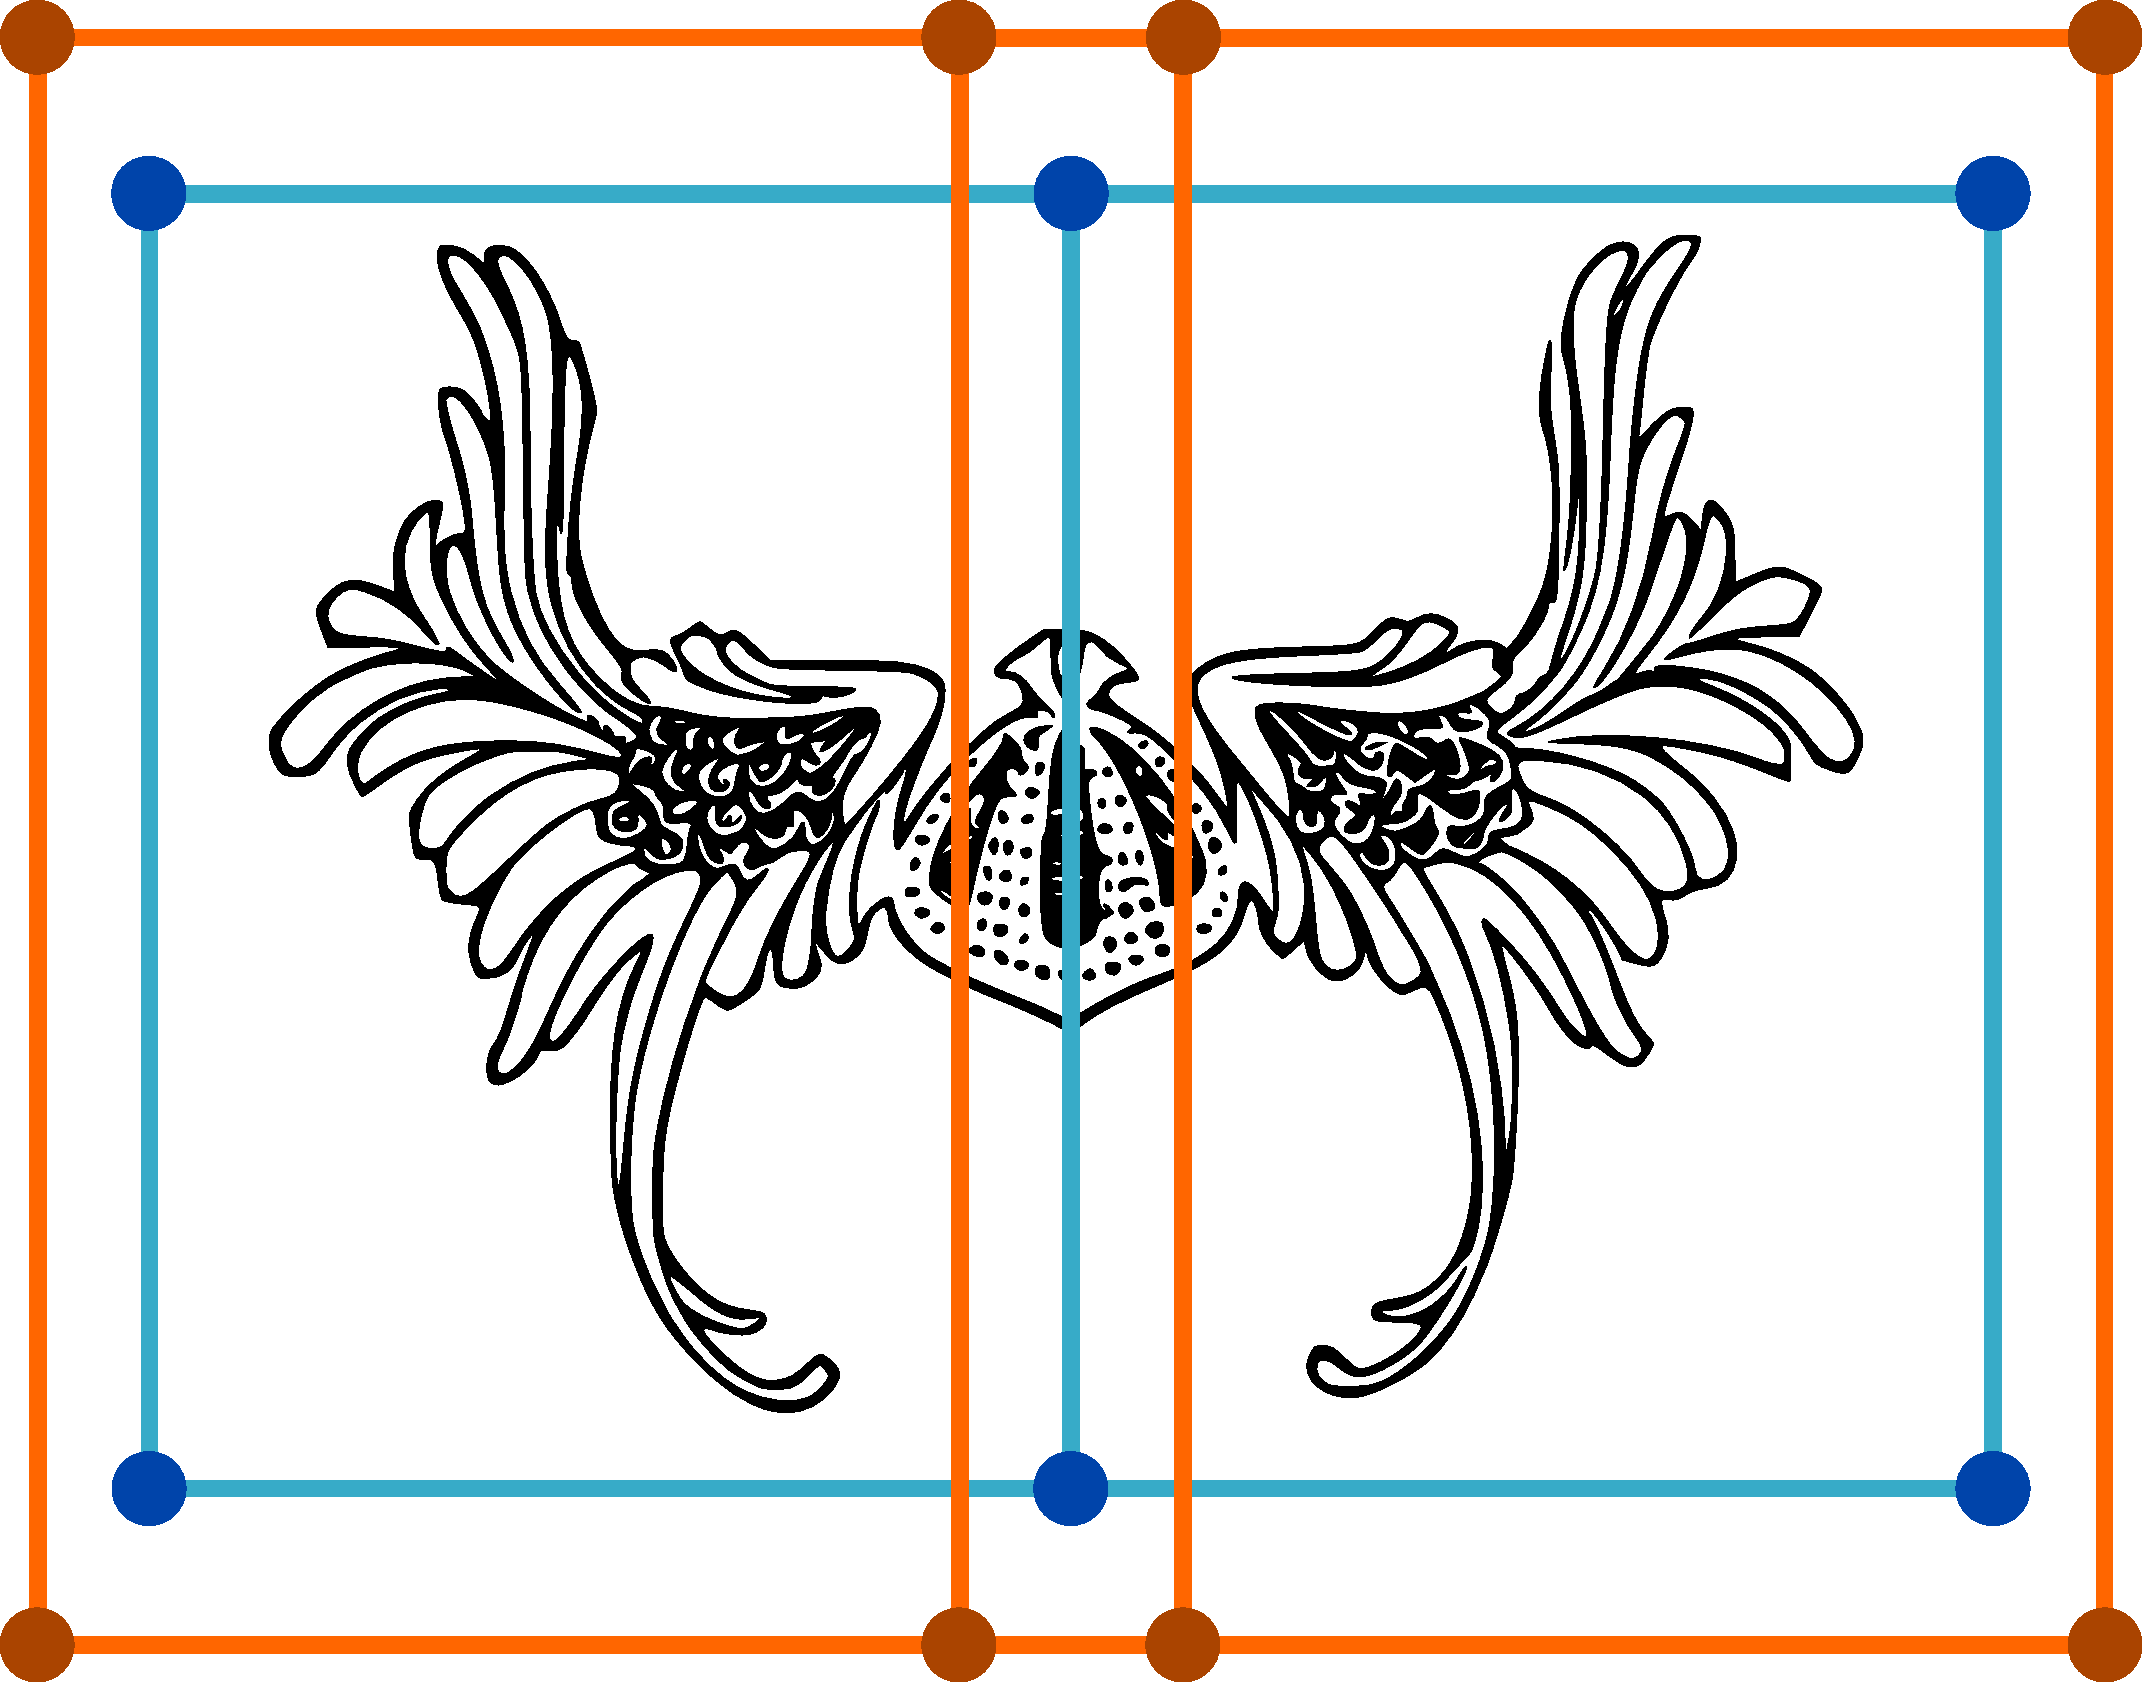
\includegraphics[scale=0.3]{Deformation-Viking-Avant}
    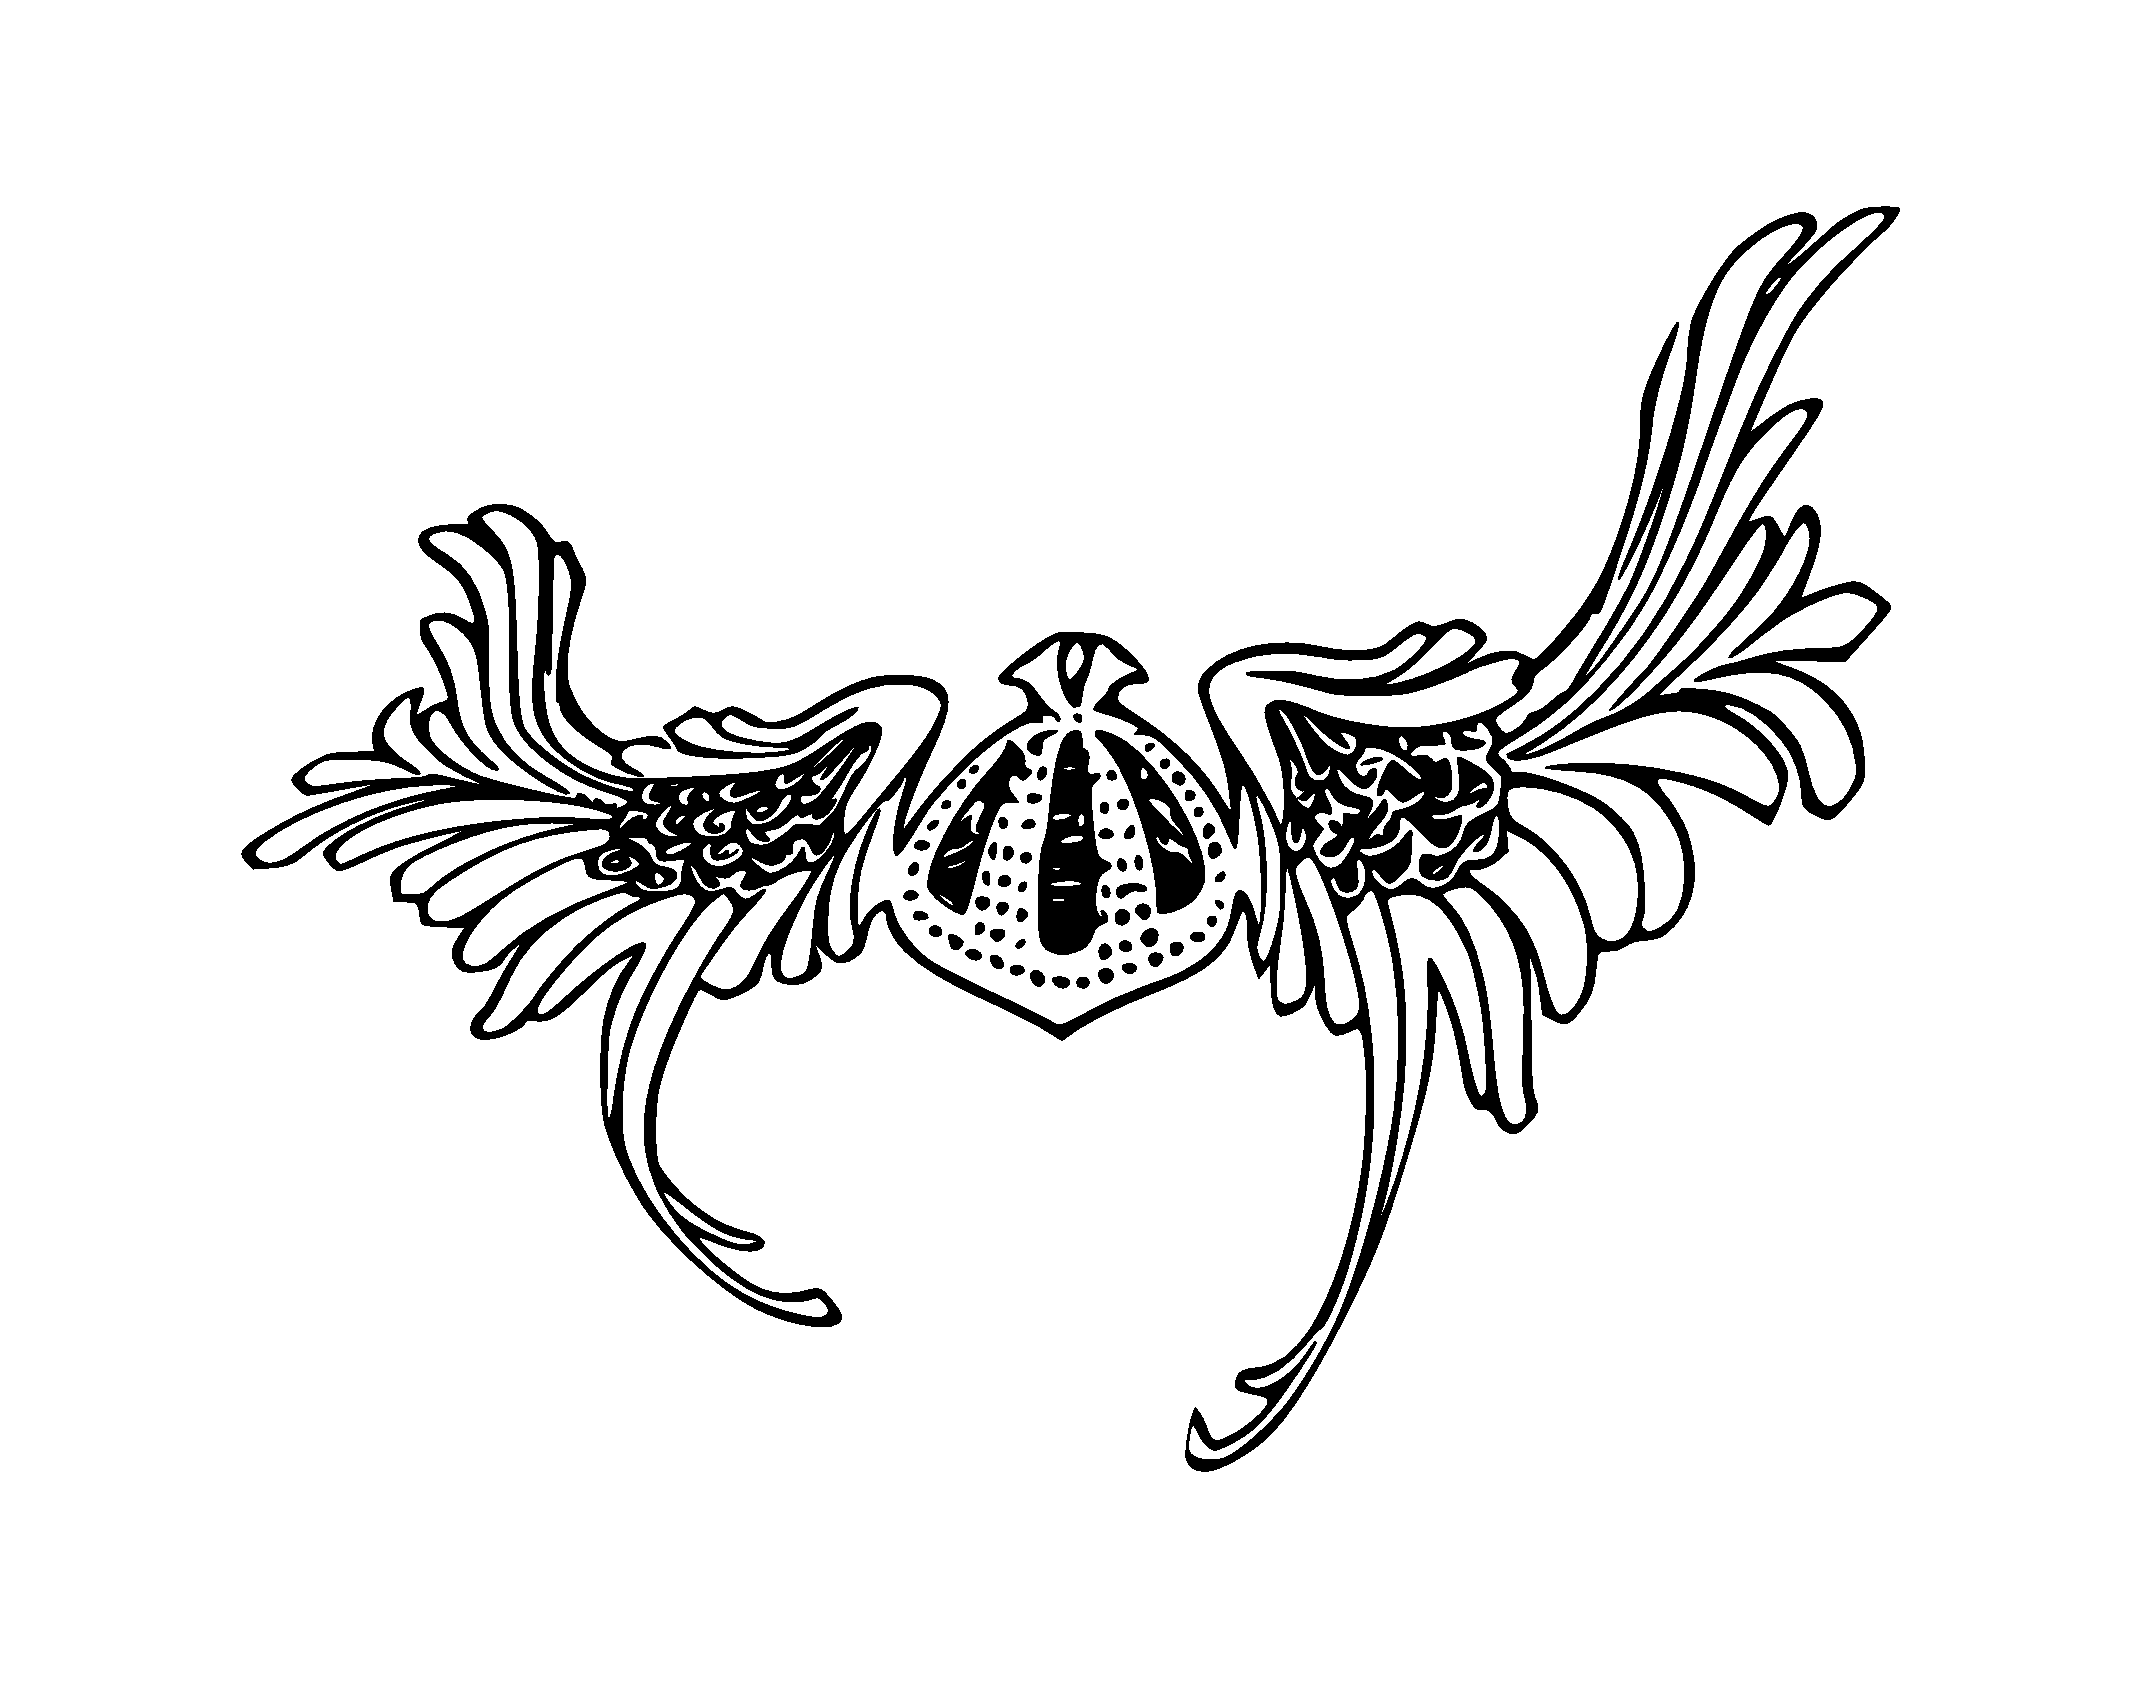
\includegraphics[scale=0.3]{Deformation-Viking-Apres}

    \caption[Exemple de déformation double-cages] {Exemple de déformation avec
deux double-cages (en bleu les cages de contrôle, en orange les cages
d'influence) où les cages de contrôle ont été collées ensembles le long d'une
arête commune. A gauche le casque avant déformation, à droite après
modification de la position des sommets des deux cages de contrôle.}

  \end{center}
\end{figure}